\chapter{Federated Learning}
\label{ch:Federated_Learning}

\section{Introduction}
In the landscape of artificial intelligence and machine learning, Federated Learning (FL)
has emerged as a paradigm that addresses key challenges related to privacy, data security,
 and decentralized computing. Federated Learning represents a novel approach to model training, allowing
 machine learning models to be trained collaboratively across multiple decentralized devices or servers
 without exchanging raw data \cite{mcmahan2023a}.

 Unlike traditional centralized approaches, where data is collected and processed in a central server, FL enables training on local devices following a scheme of decentralized model training.
 This decentralization ensures that data remains on the device, granting a certain degree of privacy.
 In a centralized setting, the trained model is updated based on the complete dataset, which is stored in a unique server. In the federated setting, data is distributed across local devices (parties or clients) and training happens locally. This can be problematic, since the source
 of the data differ, the data can differ in various ways: unbalanced datasets, different distributions, etc. This is one of the main challenges of FL:
 \textbf{non-IID data}, since this will negatively affect the performance of the model \cite{li2020}, \cite{zhao2018}, \cite{li2021}.\\
Horizontal Federated Learning (HFL) and Vertical Federated learning (VFL) are two variations of the federated learning paradigm that differ in how they distribute and collaborate on data.

\begin{itemize}
    \item \textbf{HFL:} Each party has a portion of the overall dataset, each party holds a different subset of samples but for the same features.
    \item \textbf{VFL:} The data  is vertically partitioned, each party has different features for the same set of samples.
\end{itemize}

\begin{figure}[H]
  \centering
  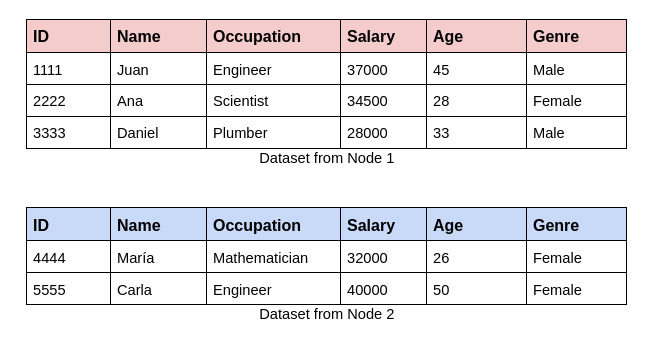
\includegraphics[width=0.6\textwidth]{figures/2-Federated_Learning/HFL.png}
  \caption{Example of HFL. Each node has different samples but with the same attributes.}
  \label{fig:HFL}
\end{figure}

\begin{figure}[h]
    \centering
    \begin{minipage}{0.40\textwidth}
        \centering
        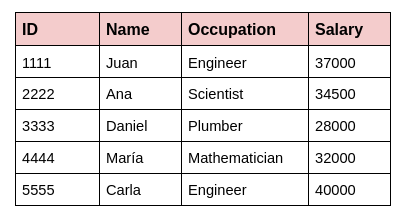
\includegraphics[width=\textwidth]{figures/2-Federated_Learning/VFL_1.png} % Primera imagen
    \end{minipage}\hspace*{2.5 em}
    \begin{minipage}{0.32\textwidth}
        \centering
        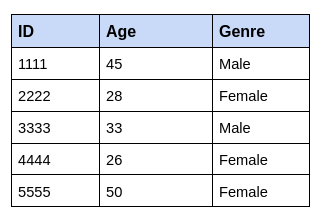
\includegraphics[width=\textwidth]{figures/2-Federated_Learning/VFL_2.png} % Segunda imagen
    \end{minipage}
    \caption{Example of VFL. Each node has common samples but with different attributes. It may happen that not all elements are common or aligned.}
    \label{fig:VFL}
\end{figure}

HFL and VFL are not mutually exclusive, in some cases a combination of both schemes may be applied. This work will focus on HFL. Also, we will only study \textit{Cross-Silo Federated Learning (Cross-Silo FL)},
which is a variation of FL that addresses the scenario where data is distributed across different organizations, usually few parties, each maintaining control over its own data.
This setting is particularly relevant in industries where different organizations need to collaborate on machine learning task, such as healthcare (hospitals collaborating on medical research), finance (banks collaborating on fraud detection), epidemiological studies (international public health agencies studying disease spread),
smart cities (urban planning authorities collaborating on public services optimization), etc. Ensuring interoperability between different silos is a huge challenge, since there needs to be a fixed standard in data format, structures and processing capabilities accross different organizations.\\
Another flavour of FL is \textit{Cross device FL}, which was the original topology proposed \cite*{mcmahan2023a}. In this type of setting, the scale of the parties is potentially much bigger (order of millions) since it's aimed to mobile devices, IoT, apps... where the data format and architecture is usually already defined by an organization. For example, this is the kind of FL that Google uses for training Gboard's models \cite*{zhang2023}. With \textit{Cross device FL}, it's needed to take into account some technical difficulties like client selection strategy \cite*{smestad2023}, connection overheard, connection dropouts, device heterogeneity, etc.
Some of these challenges are shared with \textit{Cross-Silo FL}. The main differences are the scale of parties, the computing resources (mobile devices vs data centers or computers) and the partition of data: \textit{cross device} tends to be HFL while \textit{cross-silo} could be HFL or VFL. Since we are focusing in \textit{cross-silo FL}, it won't be studied the implications of client selection (since we are assuming the parties are few and well-defined), the connection overheard or dropouts. The focus of this work will be mainly the statistical heterogeneity challenge.\\
We will begin by studying the FedAvg algorithm \cite{mcmahan2023a}, which is de facto approach for Federated Learning (FL). We will establish notation, examine some of its properties, and explore issues that arise when data is not independently identically distributed (statistical heterogeneity). Following that, various approaches that have been proposed to address this problem will be developed, and the performance of each will be analyzed across different training architectures.

\section{Objective function}

Let $D = \{(\mathbf{x}, y)\}$ be the global dataset\footnote{Here, the global dataset is the union of the different local datasets, $D = \cup_{i=1}^N D^i$ . In practical cases, there is no such dataset in order to ensure data privacy. However, we will consider it to conduct a performance study of the various algorithms.} and $D^i \subset D$ the $i$-th party's local dataset, $i=1,...,N$.
Let $\omega_g^t$ and $\omega_i^t$ be the global model and the local model of the $i$-th party in round $t\in \{1,...,T\}$, respectively. Since we are working in a \textit{Cross-silo FL} setting, the main differences between a federated optimization scheme and a distributed one would be the unbalanced data and non-IID data.\\
In a general FL optimization framework, we want to minimize the objective function:

\begin{equation}
\label{eqn:objective}
F(\omega) = \mathbb{E}_{i \sim D}\Big[ F_i (\omega_g) \Big], \qquad F_i(\omega_g) = \mathbb{E}_{z \sim D^i}\Bigl[ l_i (\omega_g, z) \Bigr]
\end{equation}

Here, $l_i(\omega_g, z)$ represents the local loss function of client i (with local dataset $D^i$). As stated in \cite*{wang2021}, the objective function in \ref{eqn:objective}
can take the form of an empirical risk minimization objective function:

\begin{equation}
  \label{eqn:empirical_objective}
  F(\omega_g) = \sum_{i=1}^N \alpha_i F_i(\omega_g) \text{ where } F_i (\omega_g) = \frac{1}{|D^i|} \sum_{z \in D^i} l_i(\omega_g, z) \text{ and } \sum_{i=1}^N \alpha_i = 1
\end{equation}

If $\alpha_i = \frac{|D^i|}{\sum_{i=1}^N |D^i|}$, the objective function in \ref{eqn:empirical_objective} would be the empirical risk minimization objective function of $D = \cup_i D^i$. We recall that \ref{eqn:objective} is an optimization problem that could be solved using Stochastic Descent: $\omega_g^{t+1} = \omega_g^t - \eta_t \nabla F (\omega_g^t)$ where $\eta_t$ is the learning rate at time $t$. In practice, we will use an unbiased estimator of the gradient of the local loss $g_i (\omega_g^t)$ such that $\mathbb{E}_{z \sim D^i} \Bigl[ g_i (\omega_g^t) \Bigr] = \nabla F_i (\omega_g^t)$ using Stochastic Gradient Descent (SGD).

\section{Statistical heterogeneity}
\label{sec:statistical_heterogeneity}

In a real-world scenario, the data distributed among parties is Non-IID, the distribution from each party differs from the global distribution. Each client has its own local optima, which may be very different from the actual global optima.
Under a IID setting, the global optima is \textit{close} to the local optima, but under a Non-IID settig, there is a \textit{drift} in the local updates, especially if the number of local epochs changes between parties.\\

In order to simulate a Non-IID setting, it has been chosen the same strategy as \cite{li2021}, the datasets will be partitioned into multiple subsets. Let the local data distribution be $P(x_i, y_i) = P(x_i|y_i)P(y_i) = P(y_i | x_i)P(x_i)$. From a distribution perspective, the following Non-IID cases summarized in \cite{kairouz2021} are considered:

\begin{itemize}
  \item \textbf{Label distribution skew:} Different $P(y_i)$ across parties.
  \item \textbf{Feature distribution skew:} Different $P(x_i)$ across parties.
  \item \textbf{Same label but different features:} Different $P(x_i | y_i)$ across parties.
  \item \textbf{Same features but different labels:} Different $P(y_i | x_i)$ across parties.
  \item \textbf{Quantity skew:} Although the parties have the same $P(x_i, y_i)$, $|D^i|$ differs.
\end{itemize}

For the \textbf{label distribution skew}, it will be used two settings. The first one, is a quantity-based label imbalance, where each party possesses data samples corresponding to a fixed number of labels. An extreme case is where each party only has data from a unique label.

\begin{figure}[H]
  \centering
  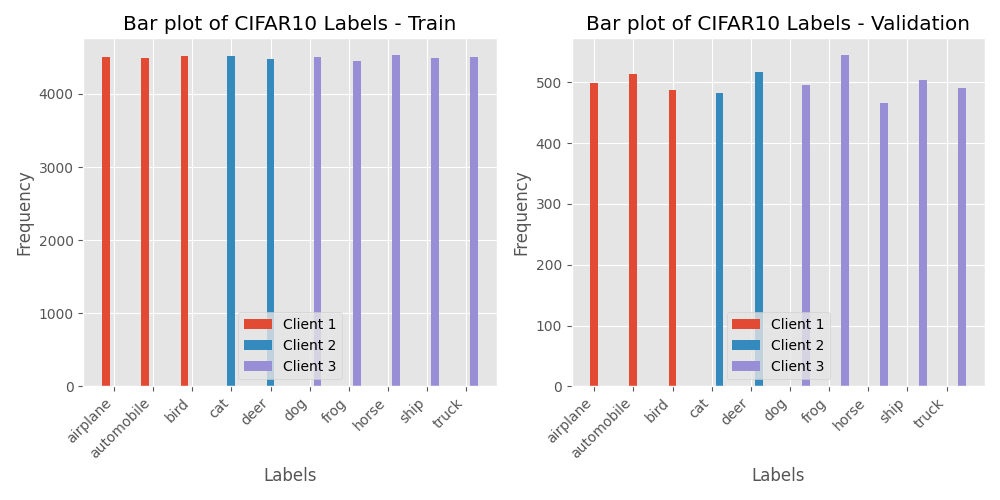
\includegraphics[width=0.6\textwidth]{figures/2-Federated_Learning/Example_Quantity_based_3_clients.png}
  \caption{Example of label distribution skew with 3 clients, each one holding data from different labels.}
  \label{fig:label_distribution_skew}
\end{figure}


The second setting is a distribution-based label imbalance, where the Dirichlet distribution $Dir(\boldsymbol{\beta})$  is used to assign different proportion of each label across parties. Given N parties, the probability density function from the Dirichlet distribution is defined as:

\begin{equation*}
  f(\mathbf{x}, \boldsymbol{\beta}) = \frac{1}{\boldsymbol{\beta}} \prod_{i=1}^N x_i^{\beta_i - 1}, \quad \sum_{i=1}^N x_i = 1, \hspace*{.3 em} x_i \in [0,1], \hspace*{.3 em} \beta_i > 0
\end{equation*}

where the normalizing constant $B(\boldsymbol{\beta})$ is the multivariate beta function.

\begin{figure}[H]
  \centering
  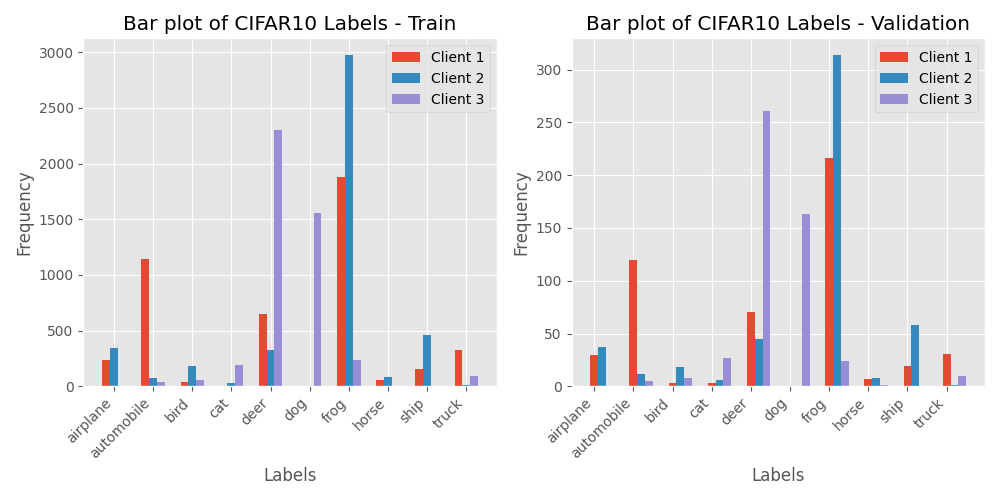
\includegraphics[width=0.6\textwidth]{figures/2-Federated_Learning/Example_Dirichlet_beta_0_5_3_clients.png}
  \caption{Example of label distribution skew with 3 clients using the Dirichlet distribution with $\boldsymbol{\beta}=(0.5, 0.5, 0.5)$.}
  \label{fig:label_distribution_skew_Dirichlet}
\end{figure}

For the \textbf{feature distribution skew}, it will be used a noise-based feature imabalance, where different levels of Gaussian noise will be added for each party. Given $\sigma > 0$, for party $i$, a noise $N(0, \sigma \frac{i}{N})$ will be added to its local features. Increasing $\sigma$ will increase the dissimilarity among parties. Note that although $P(x_i)$ differs, $P(y_i | x_i)$ is the same across parties.

\begin{figure}[!ht]
\centering
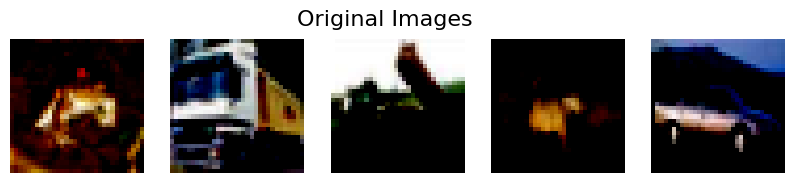
\includegraphics[width=0.4\textwidth]{figures/2-Federated_Learning/Example_noise_based_feature_imabalance_original.png}
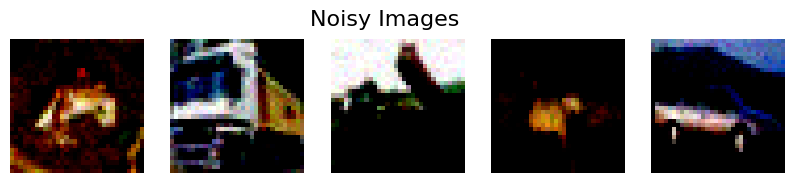
\includegraphics[width=0.4\textwidth]{figures/2-Federated_Learning/Example_noise_based_feature_imabalance_Gaussian_0.3.png}
\caption{Example of feature distribution skew with $\sigma=0.3$}
\label{fig:feature_distribution_skew_sigma_03}
\end{figure}

It will be not considered the case where $P(y_i | x_i)$ differs, because then a distributed learning setting would make no sense (same feature should be classified as a different label across parties). Different $P(x_i | y_i)$ will neither be considered since we are focusing in a Horizontal FL setting. For the quantity skew, it will be used $Dir(\boldsymbol{\beta})$ to assign different proportion of the whole dataset to each party.

\begin{figure}[H]
  \centering
  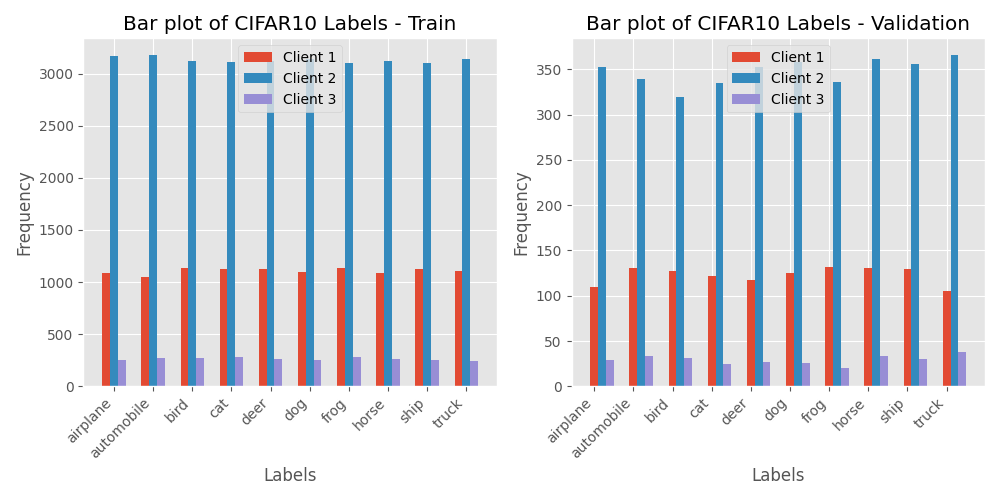
\includegraphics[width=0.6\textwidth]{figures/2-Federated_Learning/Example_Quantity_skew_3_clients.png}
  \caption{Example of quantity skew with 3 clients using the Dirichlet distribution with $\boldsymbol{\beta}=(0.5, 0.5, 0.5)$.}
  \label{fig:Quantity_skew_Dir_05}
\end{figure}

For the rest of the chapter, these Non-IID Data will be applied in order to see the effect in the model's accuracy. The model used is a very simple\footnote{The aim of these experiments is to check the accuracy degradation between different Non-IID settings. It is not necessary to train the best model in order to achieve a high test accuracy, since the IID settings will serve as a baseline to compare between Non-IID cases. Note that the number of possible experiments combining all these settings is huge, and the whole project has been made with a low-spec laptop without a GPU.} CNN described in Figure \ref{fig:CNN_used}

\begin{figure}[H]
  \centering
  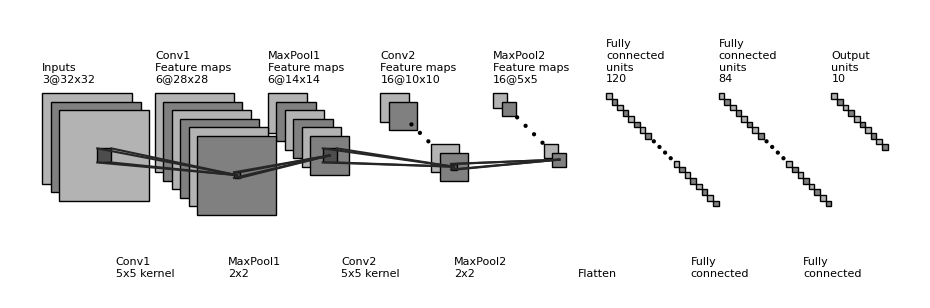
\includegraphics[width=0.6\textwidth]{figures/2-Federated_Learning/convnet_model.png}
  \caption{CNN used for all the following experiments.}
  \label{fig:CNN_used}
\end{figure}



\section{FedAvg}
In \cite*{mcmahan2023a}, it was introduced the \textbf{FederatedAveraging} algorithm (FedAvg).


\begin{algorithm}[H]
  \label{alg:FedAvg}
  \caption{FedAvg}
  \begin{algorithmic}[1]
    \Require{local datasets $D^i$ $\forall i \in \{1,\dots, N\}$, number of parties $N$, number of communication rounds $T$, number of local epochs $E$, learning rate $\eta$ for SGD, local mini-batch size $B$.}
    \Ensure{global model $\omega^T_g$.}
    \Statex
    \Procedure{Server execution}{}
    \State Initialize $\omega_g^0$
    \For {round $t = 1,\dots, T$}
      \State $S_t$  (Selection of clients)
      \For {client $k \in S_t$ \textbf{in parallel}}
        \State $\omega_k^{t+1} \gets ClientUpdate(k, \omega_g^t)$
      \EndFor
      \State $\omega_g^{t+1} \gets \sum_{k \in S_t} \frac{|D^k|}{\sum_{k \in S_t} |D^k|} \omega_k^{t+1}$
    \EndFor
    \EndProcedure

    \Procedure{$ClientUpdate(k, \omega_g^t)$}{}
    \State $\omega_k^t \gets \omega_g^t$
    \State $\mathcal{B} \gets$ Batches of $D^k$ of size $B$
    \For {local epoch $i=1,\dots,E$}
      \For {batch $\mathbf{b} \in \mathcal{B}$}
        \State $\omega_k^t \gets \omega_k^t - \eta \nabla l(\omega_k^t; \mathbf{b})$
      \EndFor
    \EndFor
    \State return $\omega_k^t$ to the server.
    \EndProcedure
  \end{algorithmic}
\end{algorithm}

As we see from Algorithm 1, \textit{FedAvg} took into account a client selection strategy. Since we are focusing in a framework where the clients are limited, we will not consider any subset of clients each round: all the clients will participate.\\
The algorithm is quite simple, the server is averaging the local models' weights, with a constant parameter determining the contribution of each client given the size of the local dataset.\\
In order to test the performance of FedAvg in different Non-IID settings, it has been used the CNN architecture described in Figure \ref{fig:CNN_used}, using CIFAR10 dataset and with a hyperparameter selection based on \cite{li2021}. First, the local metrics for each client is shown: these metrics are computed on $D^i$, for $i=1,2,3$. With each setting, $D^i$ changes and also its cardinal. How the data is partitioned is explained in section \ref{sec:statistical_heterogeneity}.
We begin with a IID setting in a 50 communication rounds FL training, each client performs only 2 local epochs and after the aggregation step, each client evaluates its model on the local test dataset, which has a similar distribution as the local train dataset (local test dataset represents the 10\% of $D^i$).

\begin{figure}[H]
  \centering
  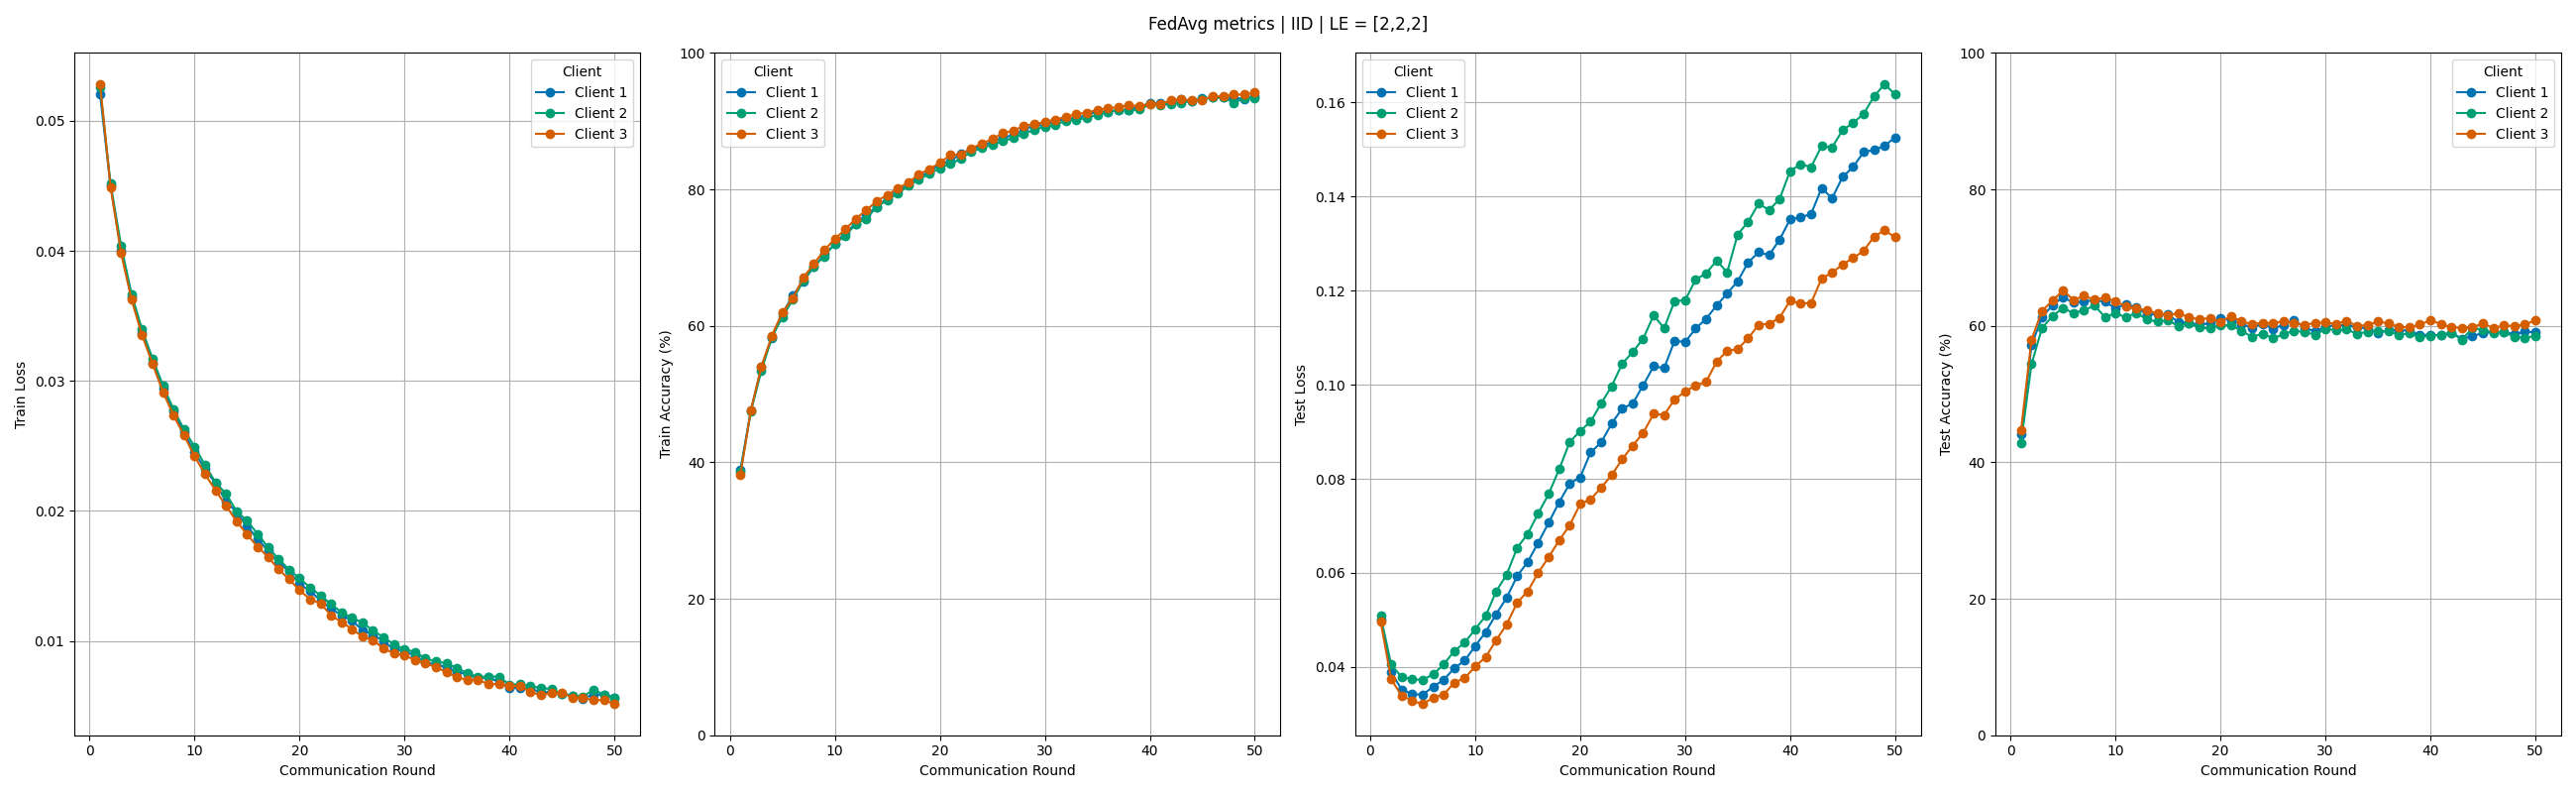
\includegraphics[width=0.9\textwidth]{figures/2-Federated_Learning/FedAvg_IID_CIFAR10_222.png}
  \caption{Local metrics for 3 clients in 50 communication rounds using FedAvg with a IID setting over the CIFAR10 dataset.}
  \label{fig:FedAvg_IID}
\end{figure}

From Figure \ref{fig:FedAvg_IID} we can see that the model converges with a local accuracy $~60\%$ for all clients and the model's behavior is similar between clients. Next experiment will simulate a Non-IID setting with label distribution skew (see Figure \ref{fig:label_distribution_skew_Dirichlet}) with $\boldsymbol{\beta} = (1,1,1)$ and 2 local epochs for each client. Given the randomness from sampling, the label distribution can change significantly between clients:

\begin{figure}[H]
  \centering
  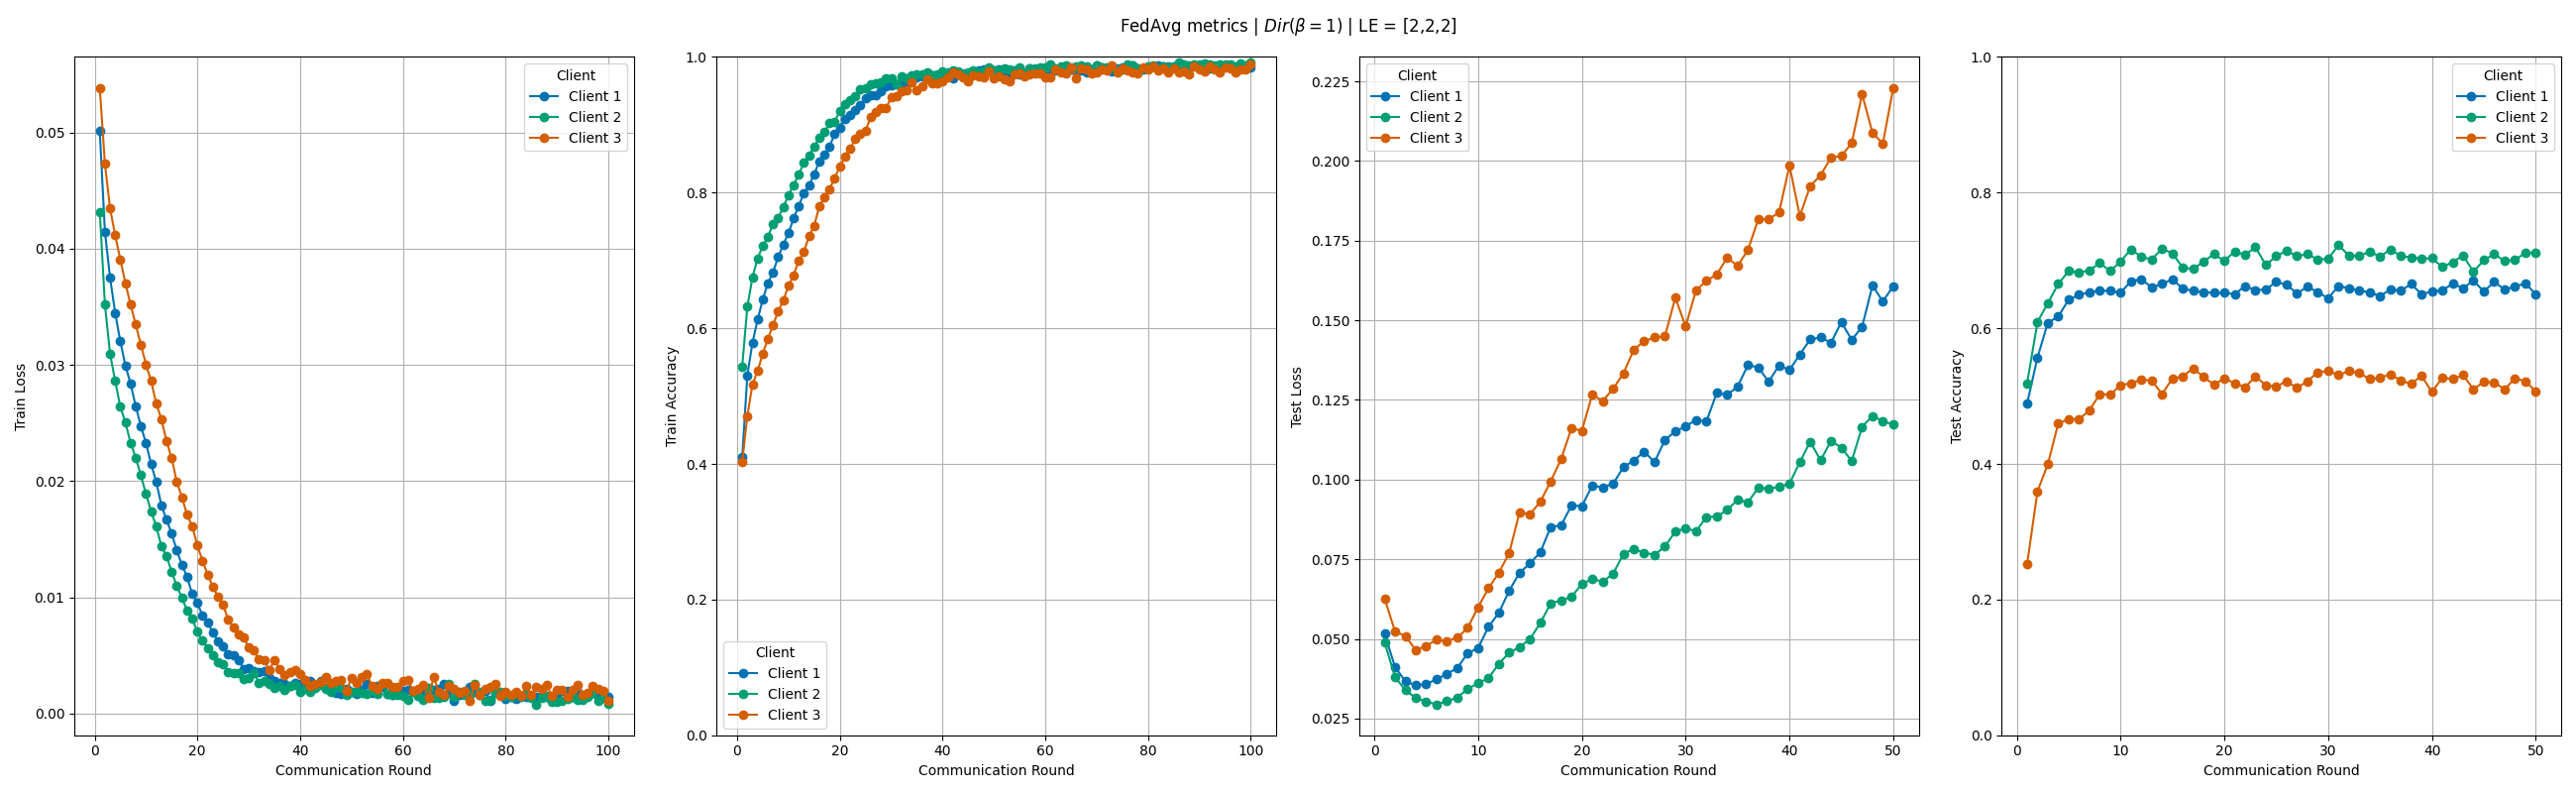
\includegraphics[width=0.9\textwidth]{figures/2-Federated_Learning/FedAvg_Dir_1_CIFAR10_222.png}
  \caption{Local metrics for 3 clients in 50 communication rounds using FedAvg with a Non-IID setting over the CIFAR10 dataset. Label distribution skew using the Dirichlet distribution with $\boldsymbol{\beta} = (1, 1, 1)$ }
  \label{fig:FedAvg_label_Dirichlet_05}
\end{figure}

From Figure \ref{fig:FedAvg_label_Dirichlet_05}, we can see that different $P(y_i)$ between clients could deteriorate the model performance, in this example, the third client had a very different distribution from the first and second client. In the aggregation step, the model deteriorates since it has been trained with a very different loss landscape.
In the next experiment, the Non-IID setting will be simulated with a Quantity skew using the Dirichlet distribution $Dir(\boldsymbol{\beta})$, $\boldsymbol{\beta} = (0.5, 0.5, 0.5)$, see Figure \ref{fig:Quantity_skew_Dir_05} for an example of this data partition.

\begin{figure}[H]
  \centering
  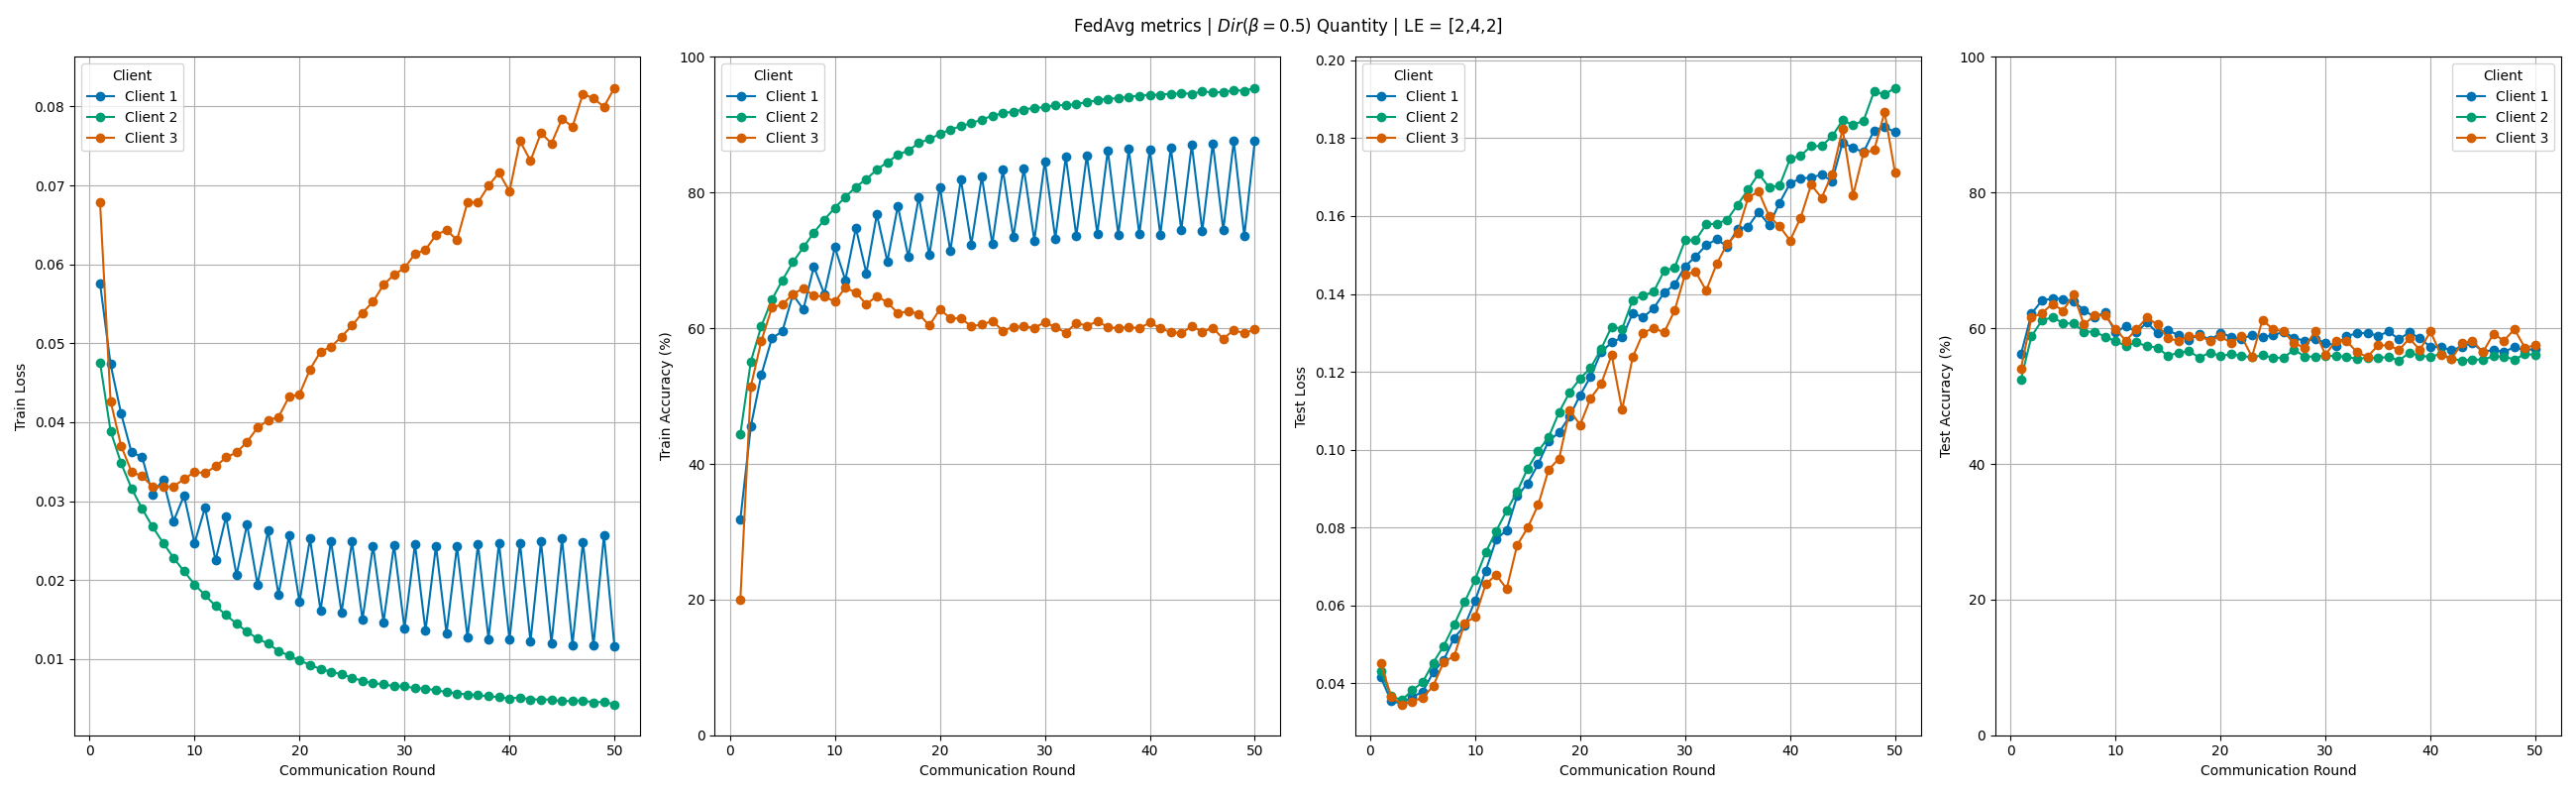
\includegraphics[width=0.9\textwidth]{figures/2-Federated_Learning/FedAvg_Dir_05_Quantity_CIFAR10_242.png}
  \caption{Local metrics for 3 clients in 50 communication rounds using FedAvg with a Non-IID setting over the CIFAR10 dataset. Quantity skew using the Dirichlet distribution with $\boldsymbol{\beta} = (0.5, 0.5, 0.5)$ }
  \label{fig:FedAvg_Quantity_Dirichlet_05}
\end{figure}

In Figure \ref{fig:FedAvg_Quantity_Dirichlet_05}, the client with more samples (client 2) has a steady training progress, while the clients with less samples (client 1 and 3) have more errors in training step, although all clients have similar performance while testing its model, therefore, the clients with less data may see an improvement participating in a FL framework when the distribution $P(x_i, y_i)$ remains the same across clients but $|D^i|$ differs.\\
Now, we'll how FedAvg handles a situation where $P(y_i)$ is different across clients (label distribution skew), see Figure \ref{fig:label_distribution_skew} for an example of this data partition. In the experiment, the first client has the first 2 labels, the second client the next 3 labels and the third client the remaining 5 labels.

\begin{figure}[H]
  \centering
  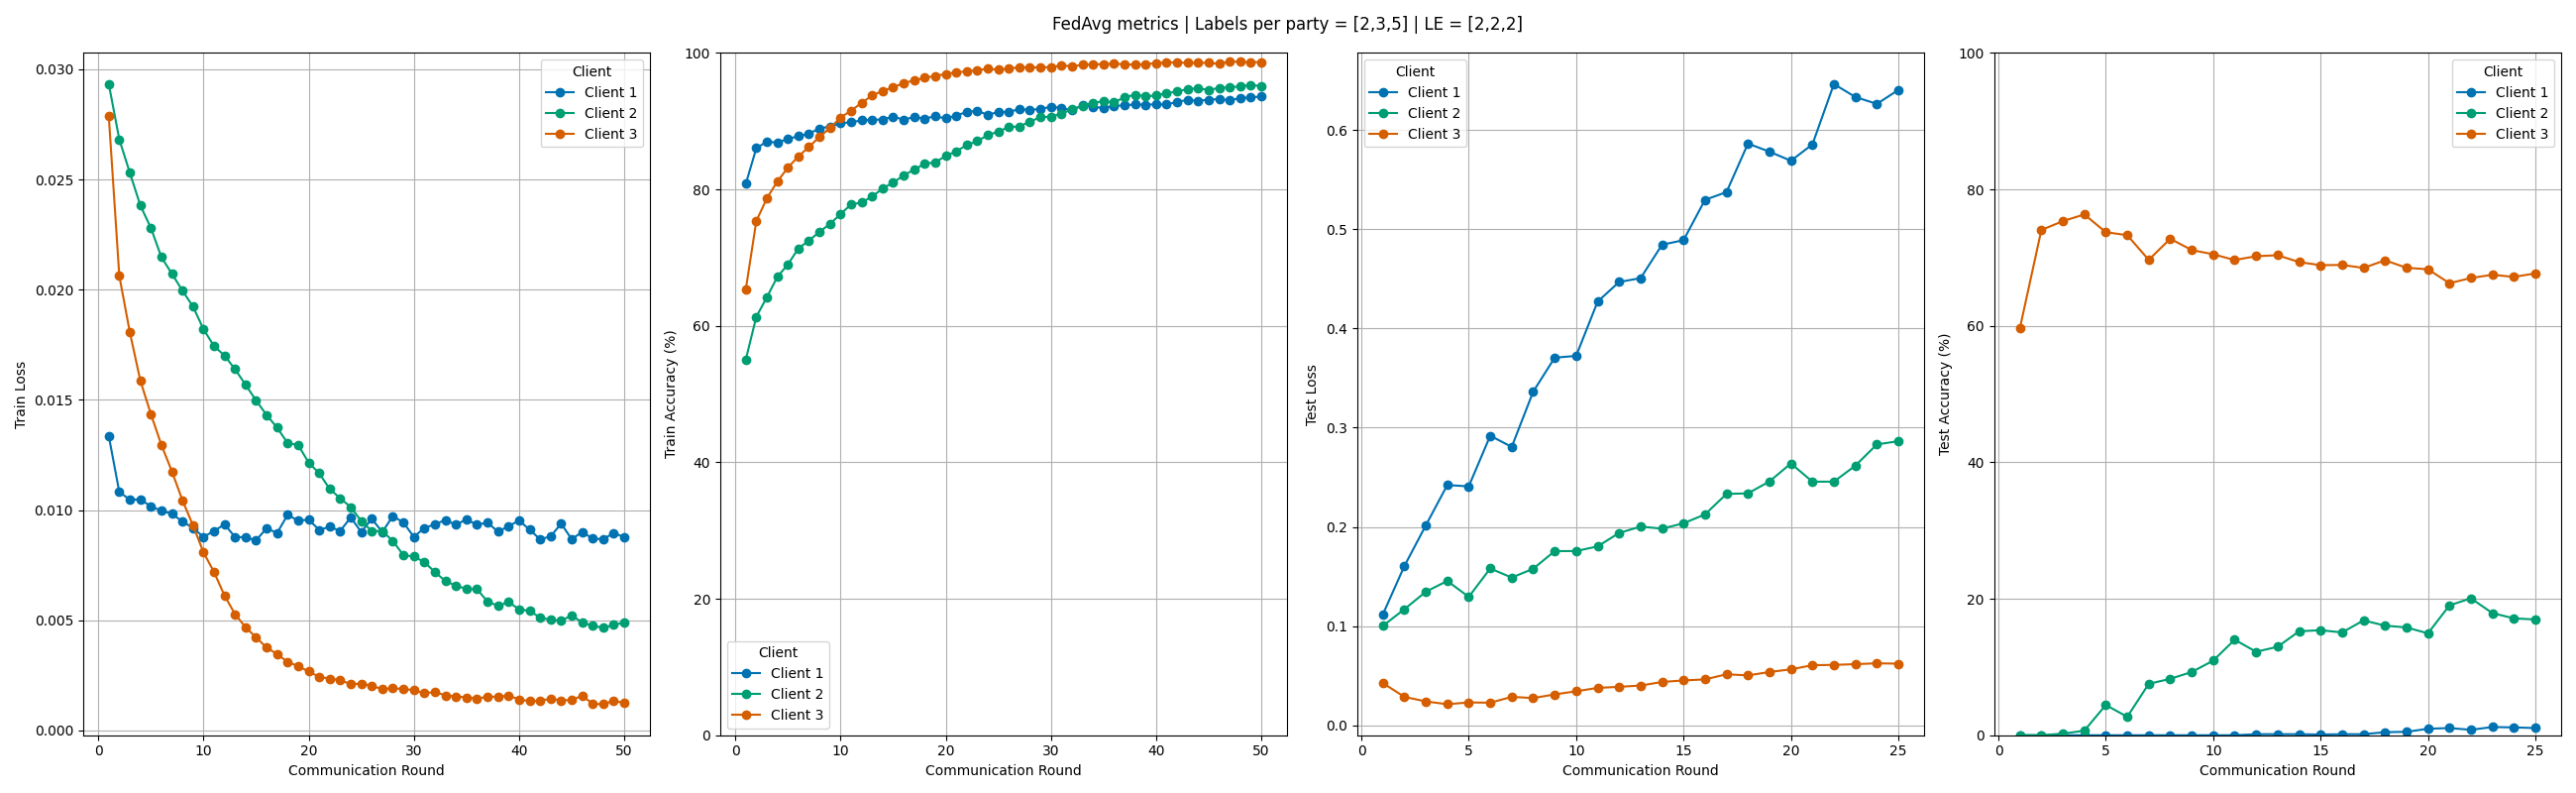
\includegraphics[width=0.9\textwidth]{figures/2-Federated_Learning/FedAvg_Label_Per_Party_235.png}
  \caption{Local metrics for 3 clients in 50 communication rounds using FedAvg with a Non-IID setting over the CIFAR10 dataset. Label distribution skew, the first client data from 2 classes, the second client from 3 classes and the third client from the 5 remaining classes.}
  \label{fig:FedAvg_Labels_Per_Party}
\end{figure}

As we can see from Figure \ref{fig:FedAvg_Labels_Per_Party}, the more labels a client has the better the performance. Since client 1 only has 2 labels, the aggregated global model doesn't classify correctly in its target domain. Recall from Algorithm \ref{alg:FedAvg} that each client's weight is proportional to its dataset's cardinal. Therefore, since client 1 has fewer data samples, this client's weights from the locally trained model looses importance against the others models.\\
For the next example, we will use the feature distribution skew, see Figure \ref{fig:feature_distribution_skew_sigma_03} for an example of this kind of assymetry using a Normal distribution $N(0, \sigma= 0.3)$. For the experiment, it will be used a $\sigma=0.5$.

\begin{figure}[H]
  \centering
  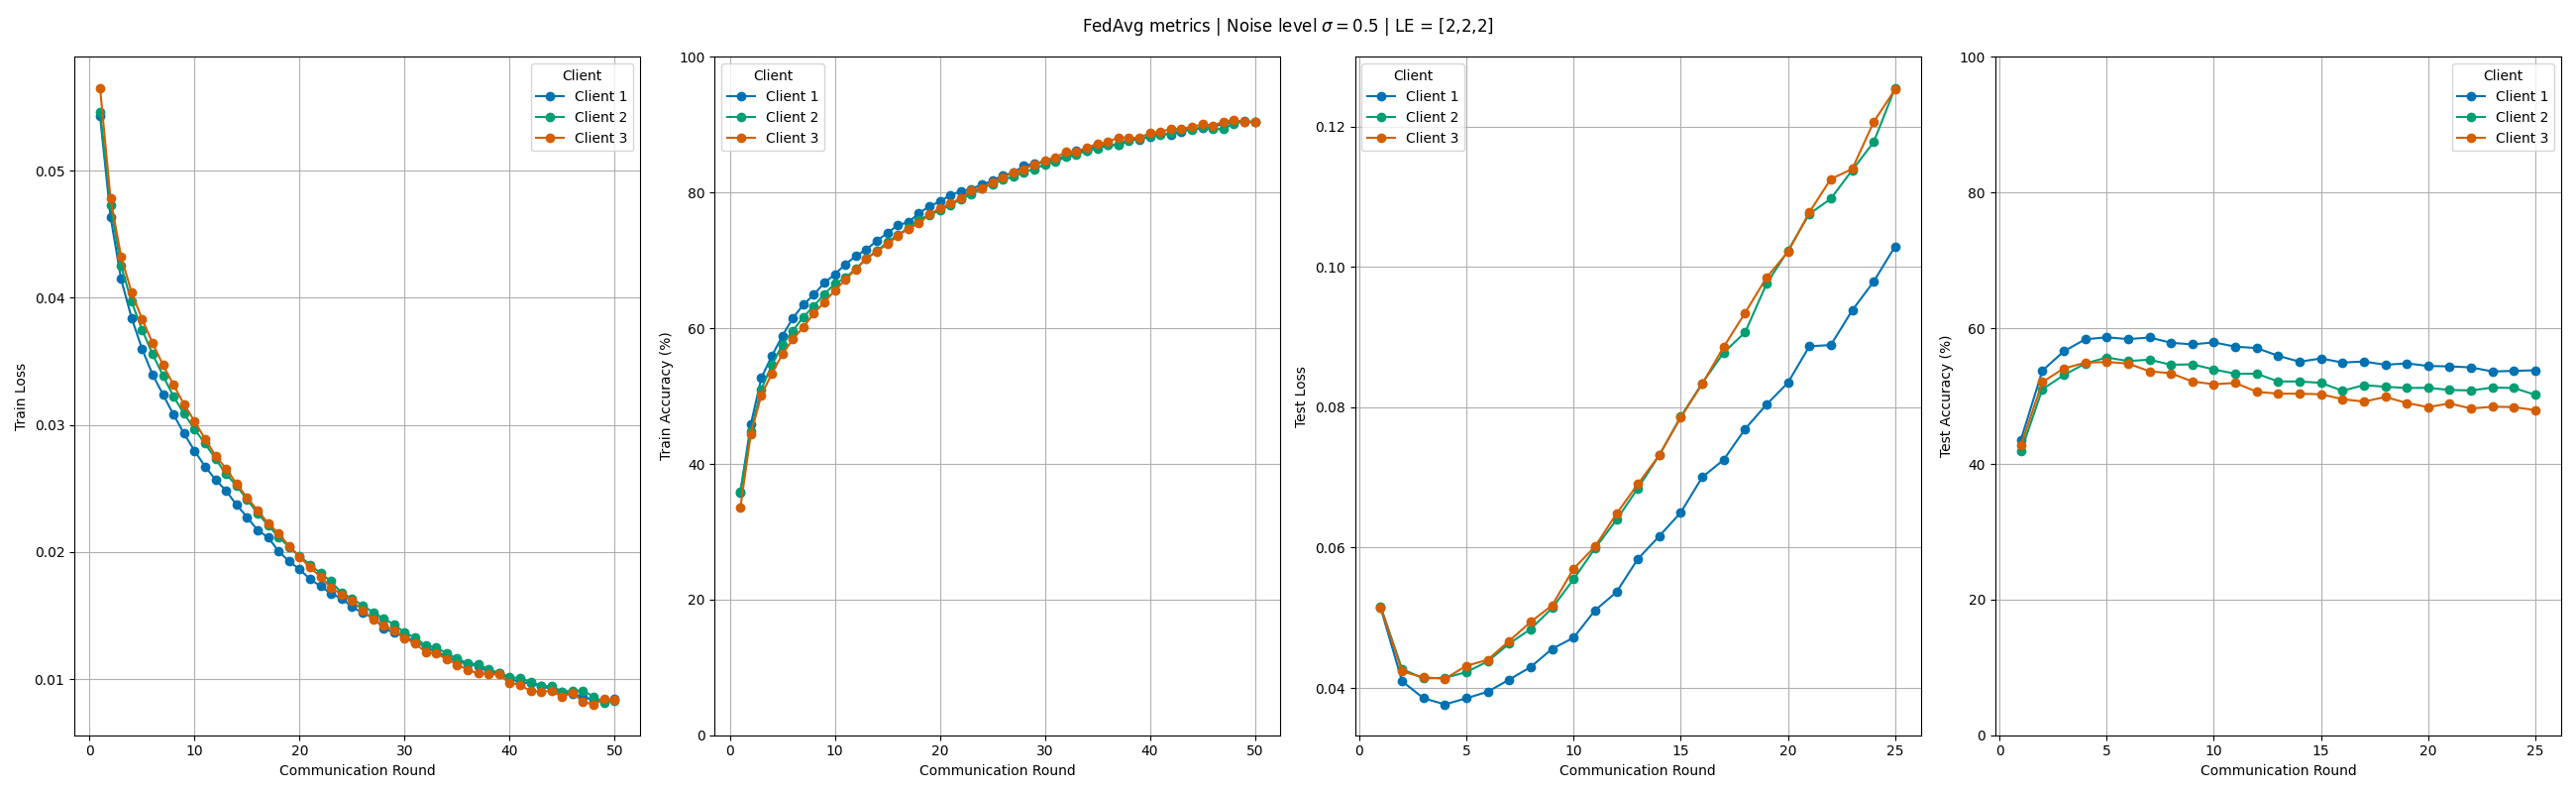
\includegraphics[width=0.9\textwidth]{figures/2-Federated_Learning/FedAvg_Noise_0.5_CIFAR10.png}
  \caption{Local metrics for 3 clients in 50 communication rounds using FedAvg with a Non-IID setting over the CIFAR10 dataset. Feature distribution skew, noise level $\sigma = 0.5$}
  \label{fig:FedAvg_Noise_level}
\end{figure}

From Figure \ref{fig:FedAvg_Noise_level} we can see that although the clients seem to converge, the model's performance is worst in comparison with a IID setting.\\
Even though in a real scenario there wouldn't be a global test dataset, a comparison between different data partition settings in addition to a centralized training scenario will be tested with the union of all clients' datasets. This will serve to see how good the global model performs in comparison with a centralized model.

\begin{figure}[H]
  \centering
  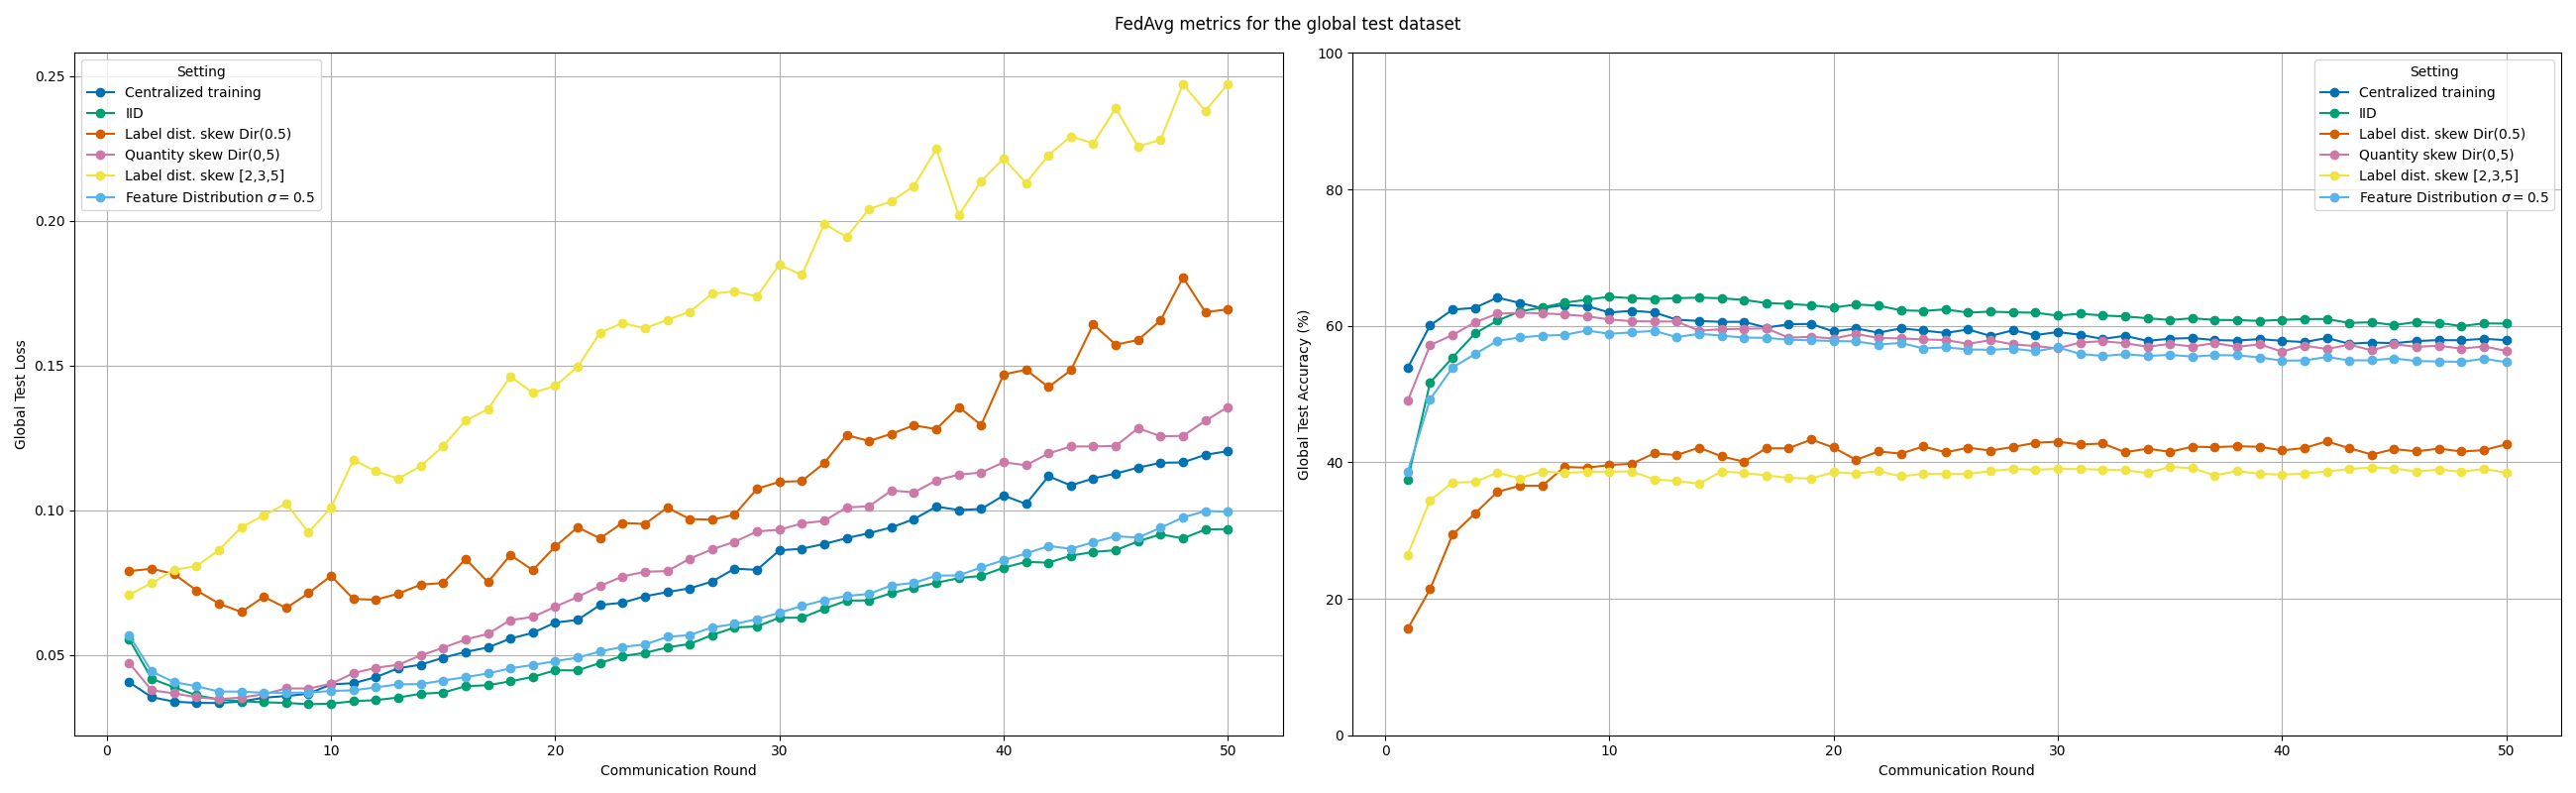
\includegraphics[width=0.8\textwidth]{figures/2-Federated_Learning/FedAvg_central_metrics.png}
  \caption{Test metric for different data distribution settings using (theoretical) global dataset $D$ compared with a centralized setting.}
  \label{fig:FedAvg_Central_Metrics}
\end{figure}

As it can be seen from Figure \ref{fig:FedAvg_Central_Metrics}, the centralized, IID, quantity skew and feature distribution skew settings perform quite similar, being both label distribution skew settings the ones that degrades the model the most. From Algorithm \ref{alg:FedAvg}, each client performs multiple local epochs, which reduces the communication rounds. However, these local updates can lead to a worse performance since the local objective functions differ from each other. This makes the algorithm not robust against non-IID data. There are several works that try to tackle this problem and a lot of FedAvg variants have been proposed in order to mitigate the divergence between the local updates. We will review some of the more relevant of them, starting with \textit{FedProx}.

\section{FedProx}

In \cite*{li2020}, a generalization of \textit{FedAvg} was proposed where the local function to minimize $F_k(\omega_k)$ was modified adding a proximal term:

\begin{equation}
  \min_{\omega_k} h_k (\omega_k, \omega_g^t) = F_k(\omega_k) + \frac{\mu}{2} \lVert \omega_k - \omega_g^t \rVert^2, \qquad \mu \geq 0
\end{equation}

The basic idea, is to restrict the local updates to be closer to the actual global model. In the original proposal, it was stated that a constant number of local epochs per round each time could be not feasible because of the device / system heterogeneity. Since this work is not focused on system heterogeneity, it will not be mentioned the theoretical convergence results.

\textit{FedAvg} is a particular case when $\mu = 0$, a fixed number of local epochs $E$ is set and all the local solvers are SGD. As $\mu$ increases, the function becomes more restrictive meaning that it will take longer to converge. This algorithm doesn't restrict us to any local solver, so it's not necessary to compute the estimation of the gradient using SGD.
When the data across clients is IID, a positive $\mu$ could decelerate the convergence, some heuristics could be applied such as decreasing $\mu$ as long as the loss functions continues to decrease. Following the experiments in \cite*{li2020}, the possible values of $\mu$ that will be used in this work are selected from the finite set $\{0.001, 0.01, 0.1, 1\}$

\begin{figure}[H]
    \centering

    \begin{subfigure}{\linewidth}
        \centering
        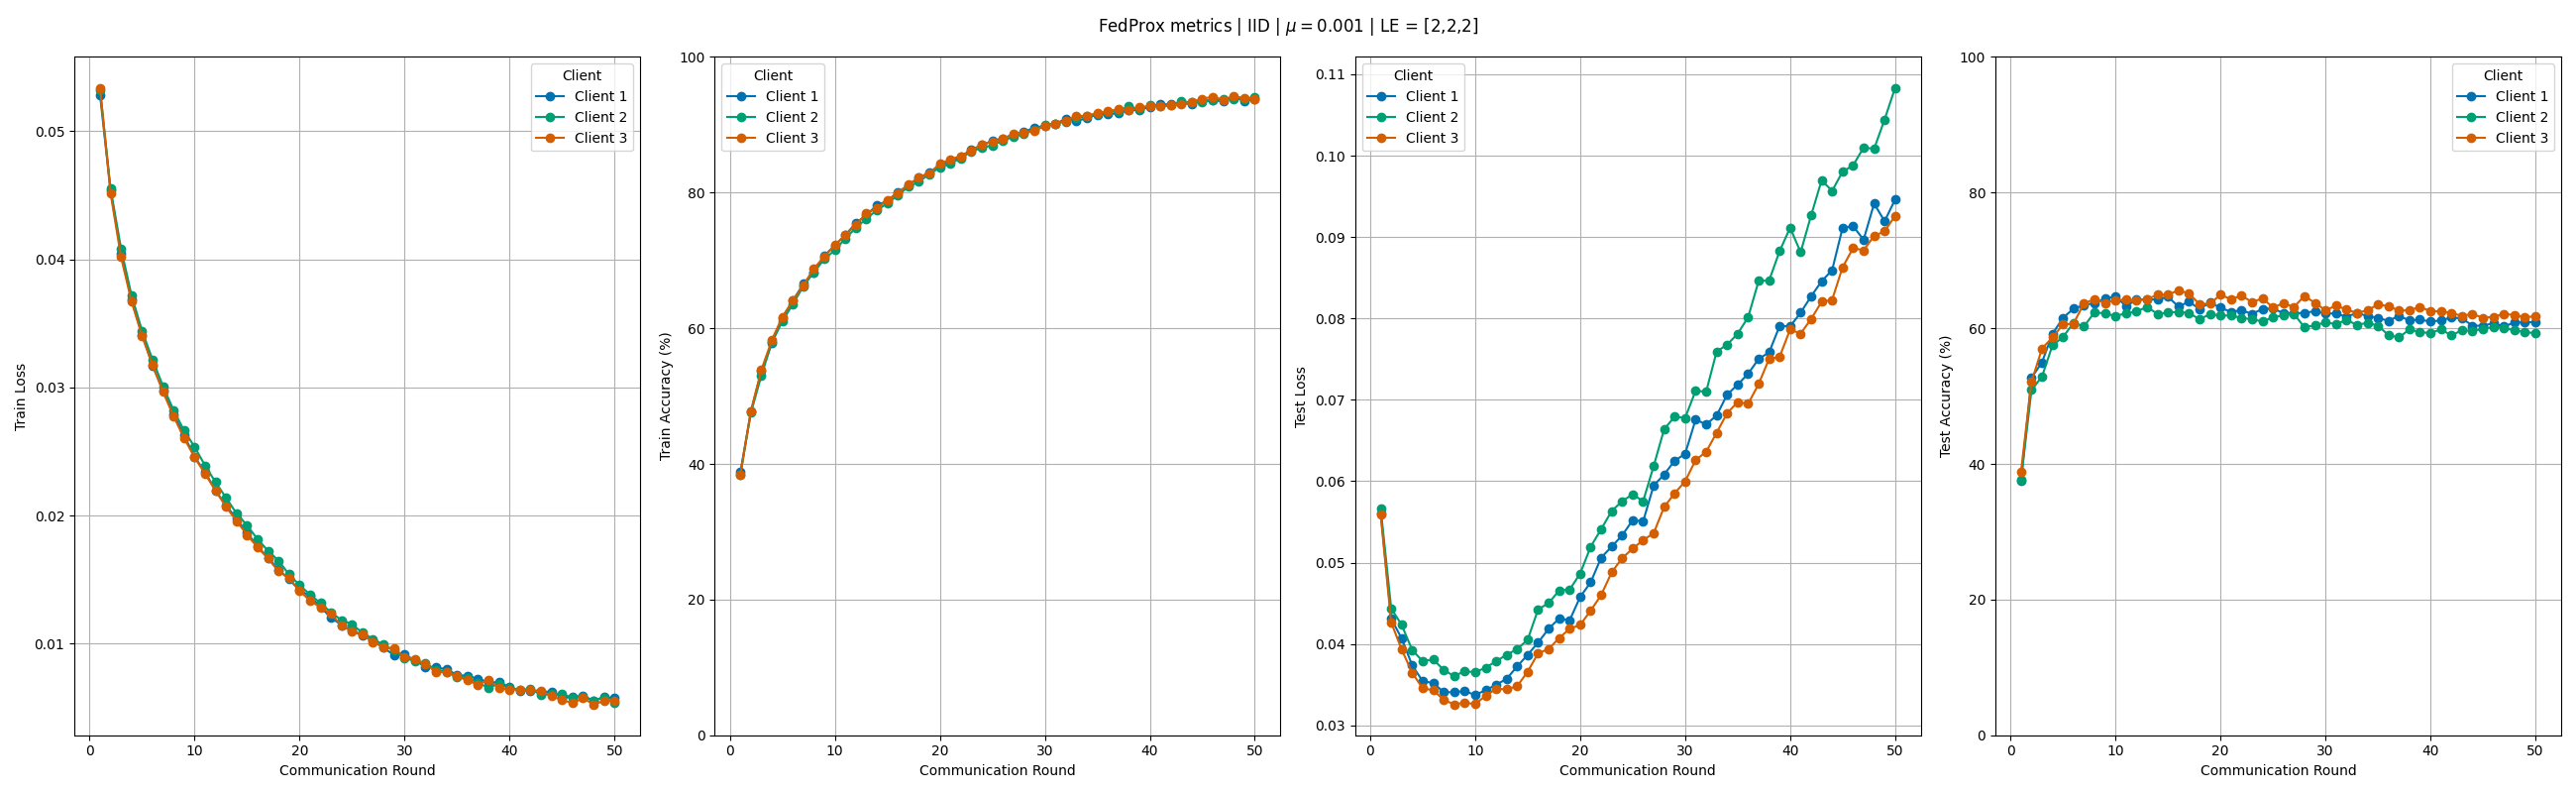
\includegraphics[width=0.8\linewidth]{figures/2-Federated_Learning/FedProx_IID_Mu_0.001.png}
    \end{subfigure}
    \vspace{1em} % Space between images

    \begin{subfigure}{\linewidth}
        \centering
        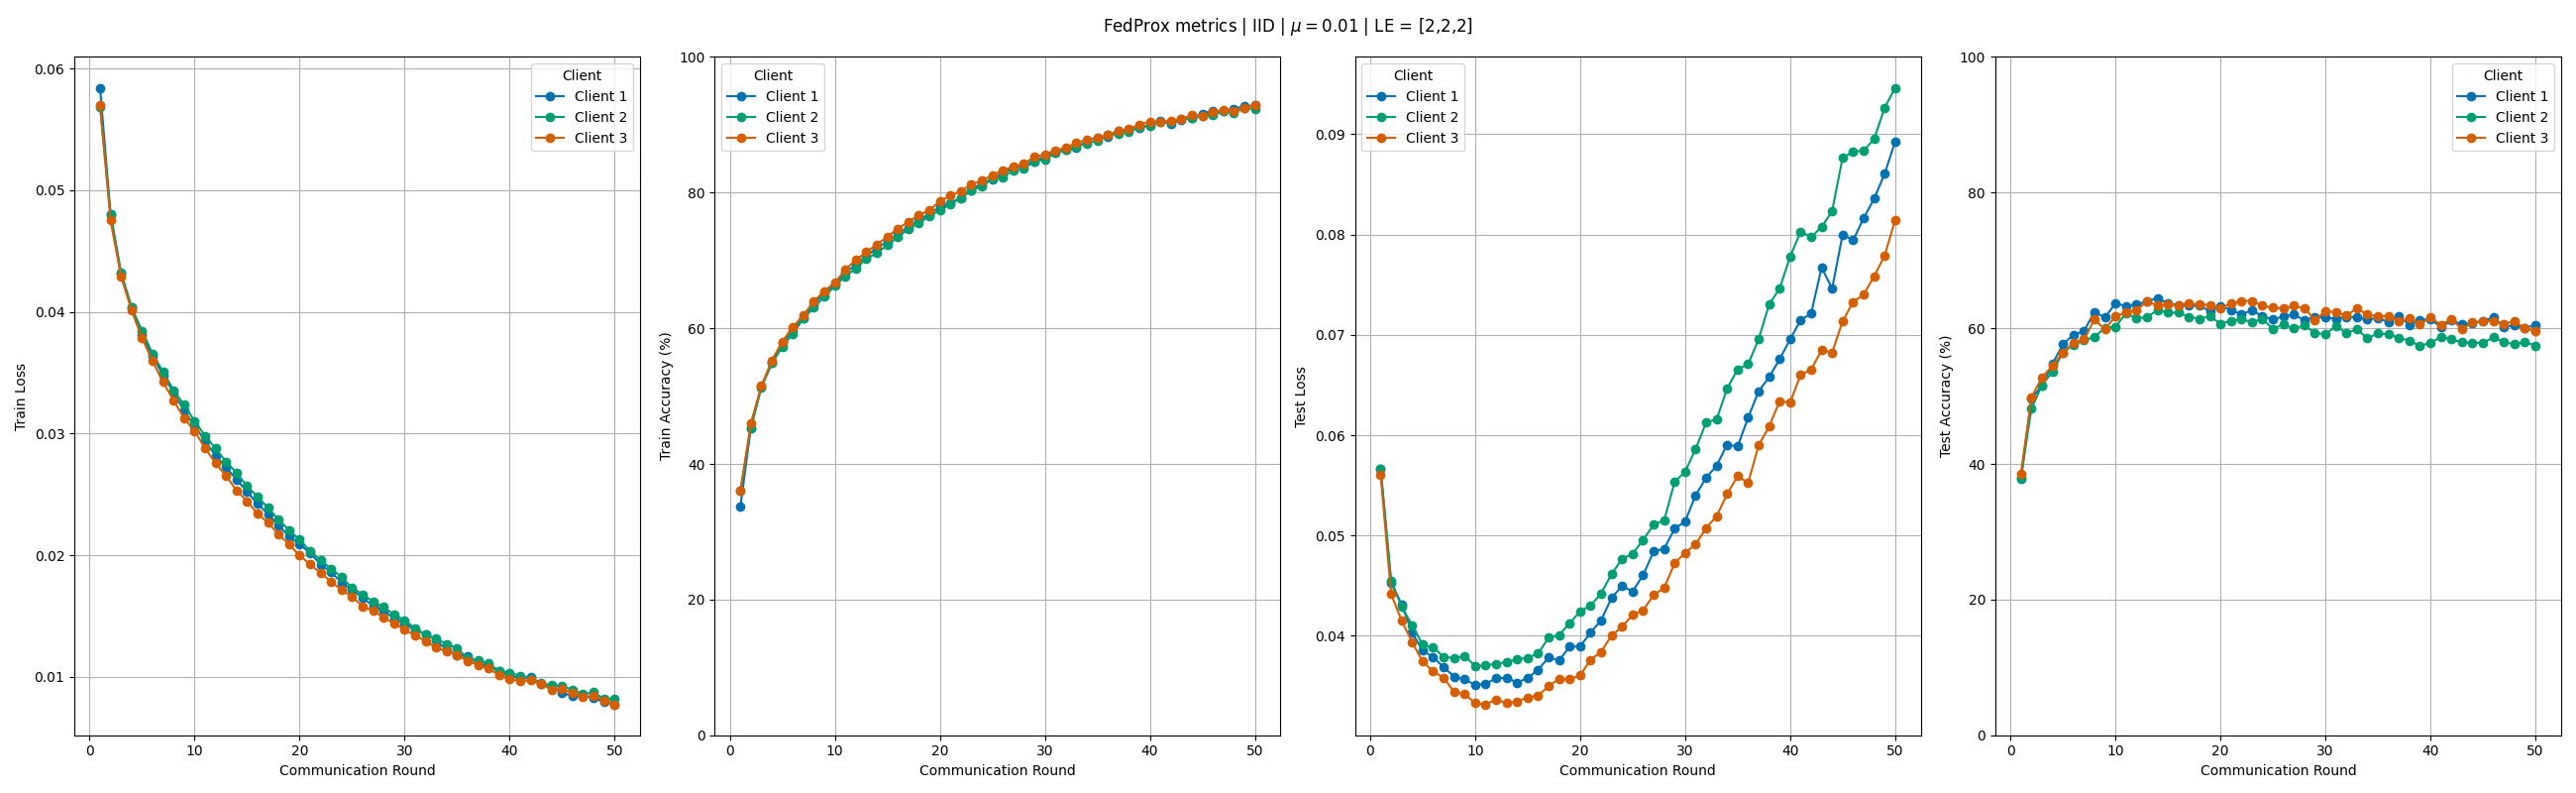
\includegraphics[width=0.8\linewidth]{figures/2-Federated_Learning/FedProx_IID_Mu_0.01.png}
    \end{subfigure}
    \vspace{1em} % Space between images

    \begin{subfigure}{\linewidth}
        \centering
        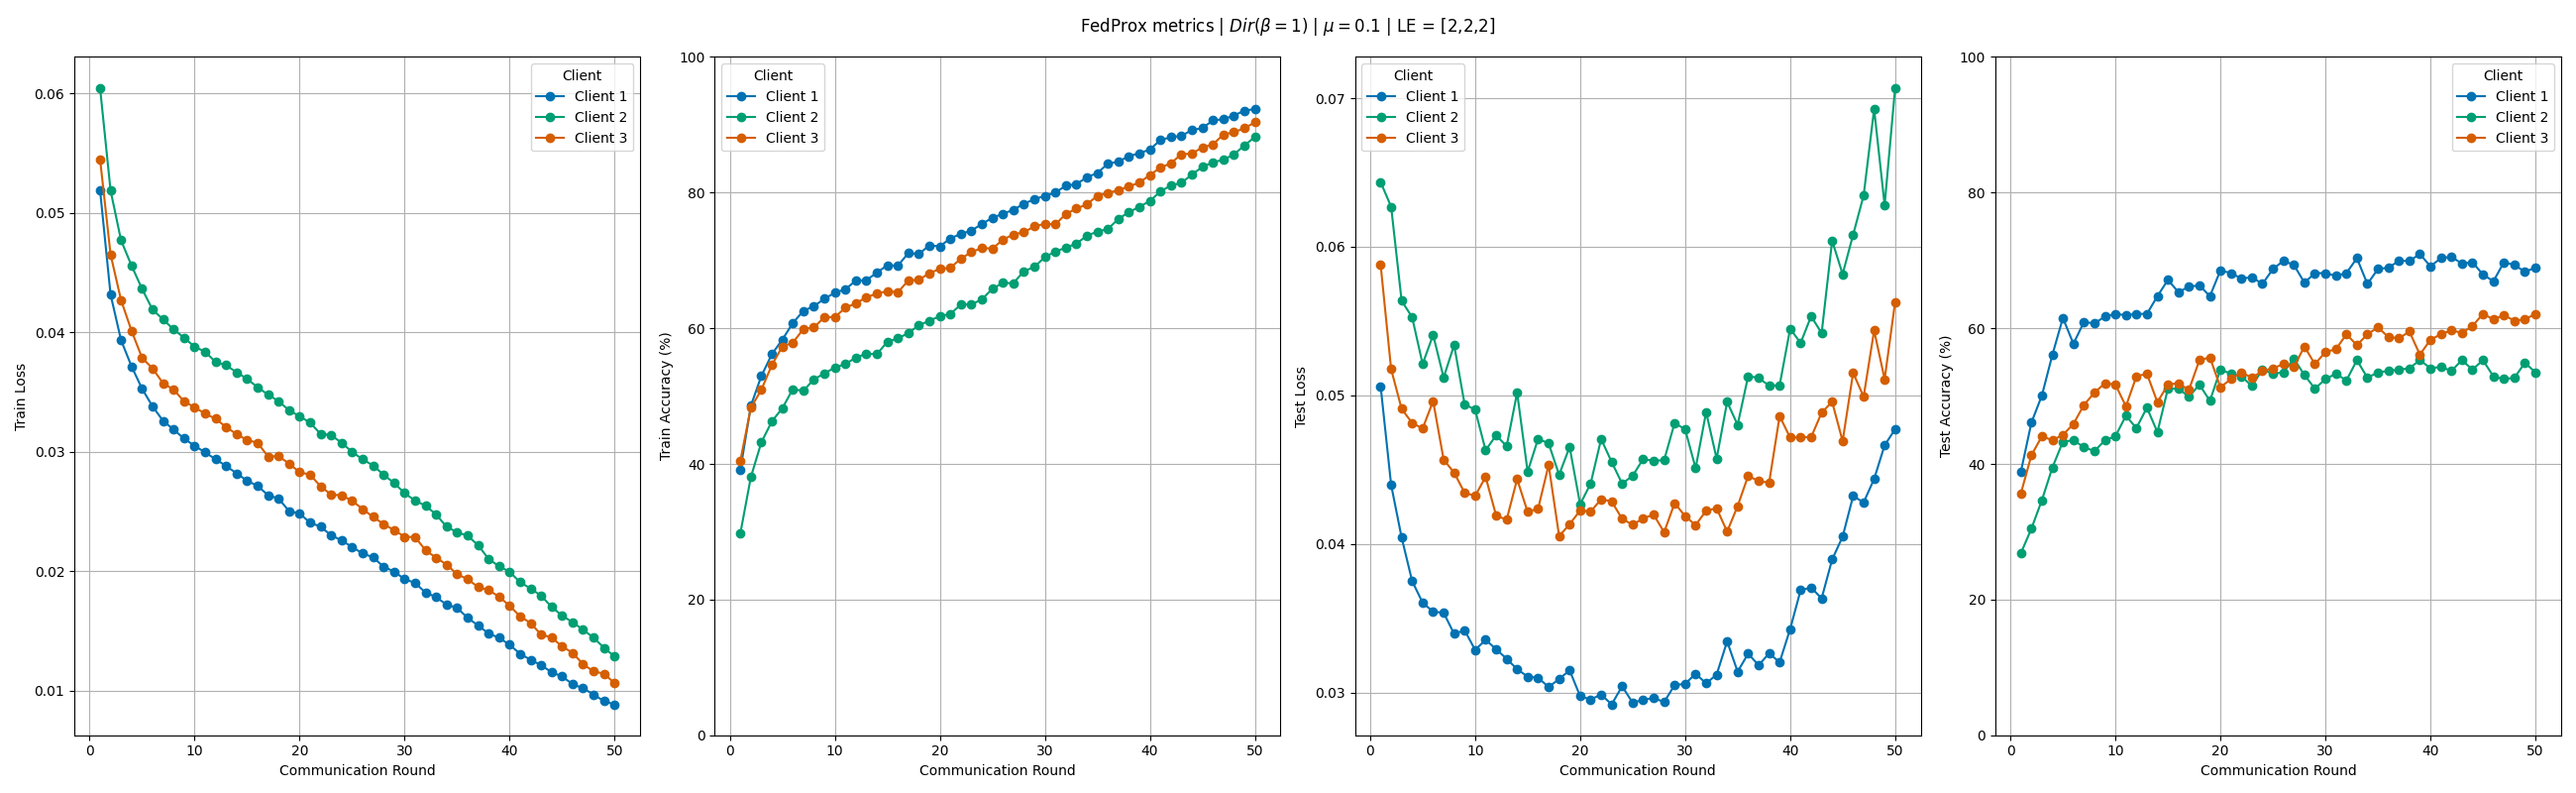
\includegraphics[width=0.8\linewidth]{figures/2-Federated_Learning/FedProx_Dirichlet_1_mu_0.1.png}
    \end{subfigure}
    \vspace{1em} % Space between images

    \begin{subfigure}{\linewidth}
        \centering
        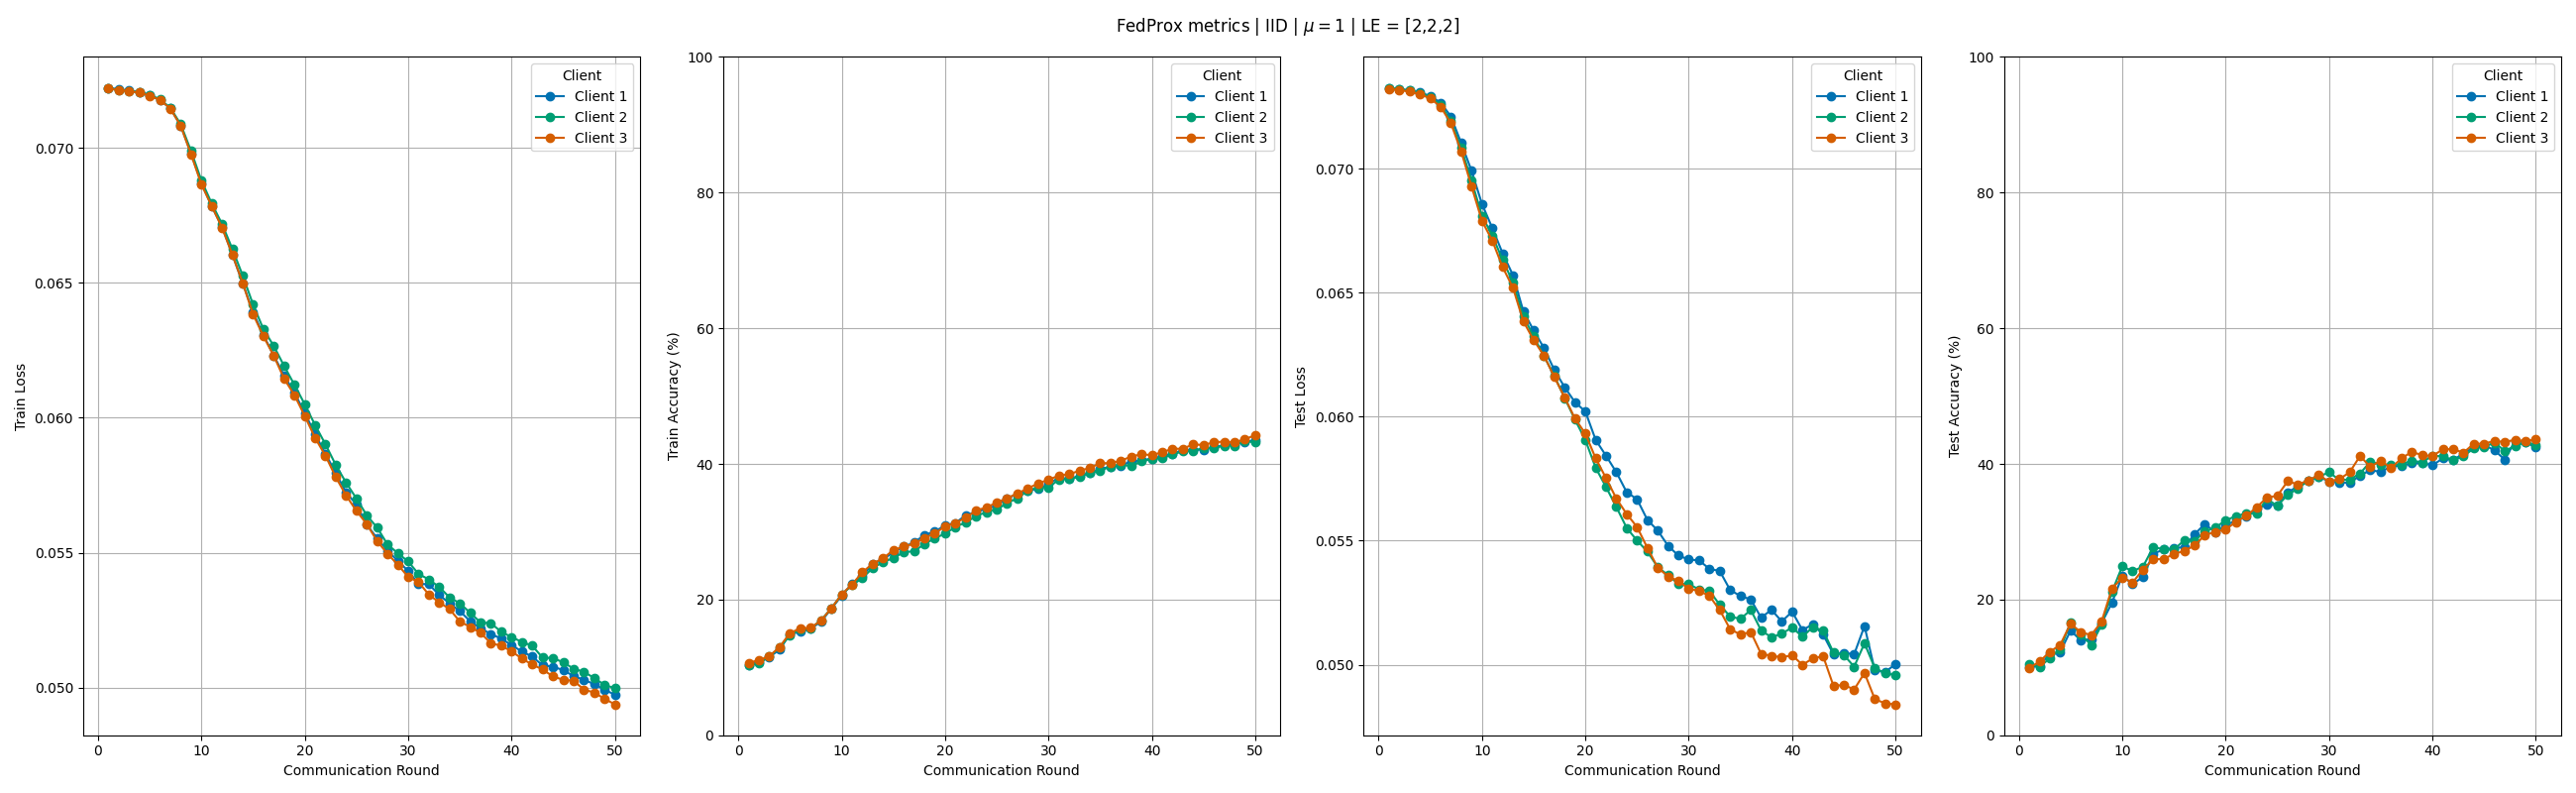
\includegraphics[width=0.8\linewidth]{figures/2-Federated_Learning/FedProx_IID_Mu_1.png}
    \end{subfigure}

    \caption{Local metrics for 3 clients in 50 communication rounds using FedProx with a IID setting over the CIFAR10 dataset, $\mu \in \{0.001, 0.01, 0.1, 1\}$}
    \label{fig:FedProx_IID}
\end{figure}

Seeing Figure \ref{fig:FedAvg_Quantity_Dirichlet_05}, according to \cite*{li2020} and \cite*{li2021}, A larger $\mu$  could decrease the model's convergence even in an IID setting. As of today, only heuristics are available to choose $\mu$; some of them consist of reducing the parameter as training progresses, similar to adjusting the learning rate. The rest of Non-IID setting experiments metrics with FedProx can be seen in Appendix A, for the label distribution skew using $Dir(\boldsymbol{\beta} = (1,1,1))$ see Figure \ref{fig:FedProx_Non_IID_Dirichlet_1}, for a label distribution skew with different labels per party see Figure \ref{fig:FedProx_Non_IID_LabelsPerParty}, for a label quantity distribution skew using $Dir(\boldsymbol{\beta}=(0.5,0.5,0.5))$ see Figure \ref{fig:FedProx_Non_IID_LabelQuantitySkeqDir_05} and for a feature distribution skew with noise level $\sigma = 0.5$ see Figure \ref{fig:FedProx_Non_IID_NoiseLevel_05}.\\
Now only a few cases will be shown where with different values of mu a similar or better result has been obtained compared to FedAvg under the same conditions.

\begin{figure}[H]
  \centering
  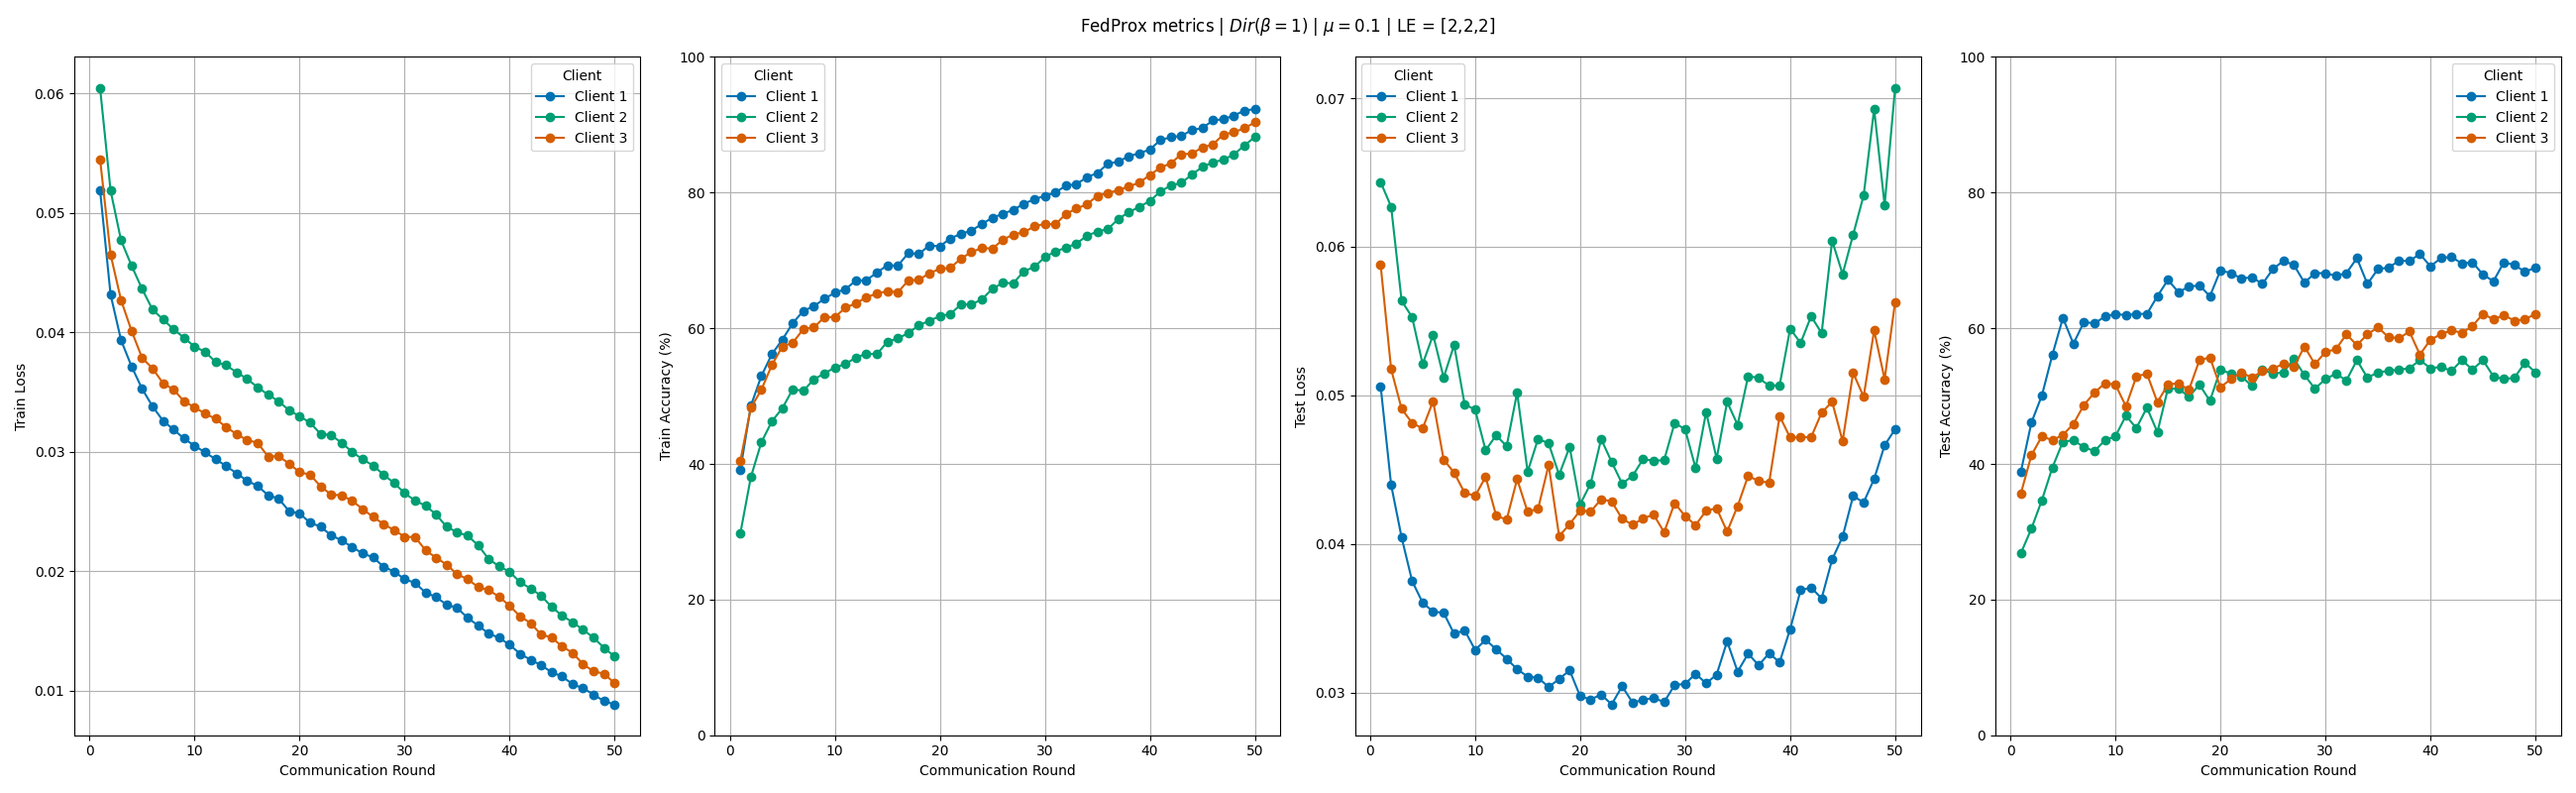
\includegraphics[width=0.8\textwidth]{figures/2-Federated_Learning/FedProx_Dirichlet_1_mu_0.1.png}
  \caption{Local metrics for FedProx, $\mu = 0.1$, label distribution skew using $Dir(\boldsymbol{\beta})$, $\boldsymbol{\beta} = (1,1,1)$}
  \label{fig:FedProx_LabelsSkewDir_1_Mu_0.1}
\end{figure}

Comparing Figure \ref{fig:FedAvg_label_Dirichlet_05} and Figure \ref{fig:FedProx_LabelsSkewDir_1_Mu_0.1} we can see that the clients' local training improves slightly, specially for client 2 and 3. However, we will compare both models using the global dataset $D$ in order to test if it hasn't been overfitted by a client whose local dataset's cardinal is way bigger that the rest of clients.

\begin{figure}[H]
  \centering
  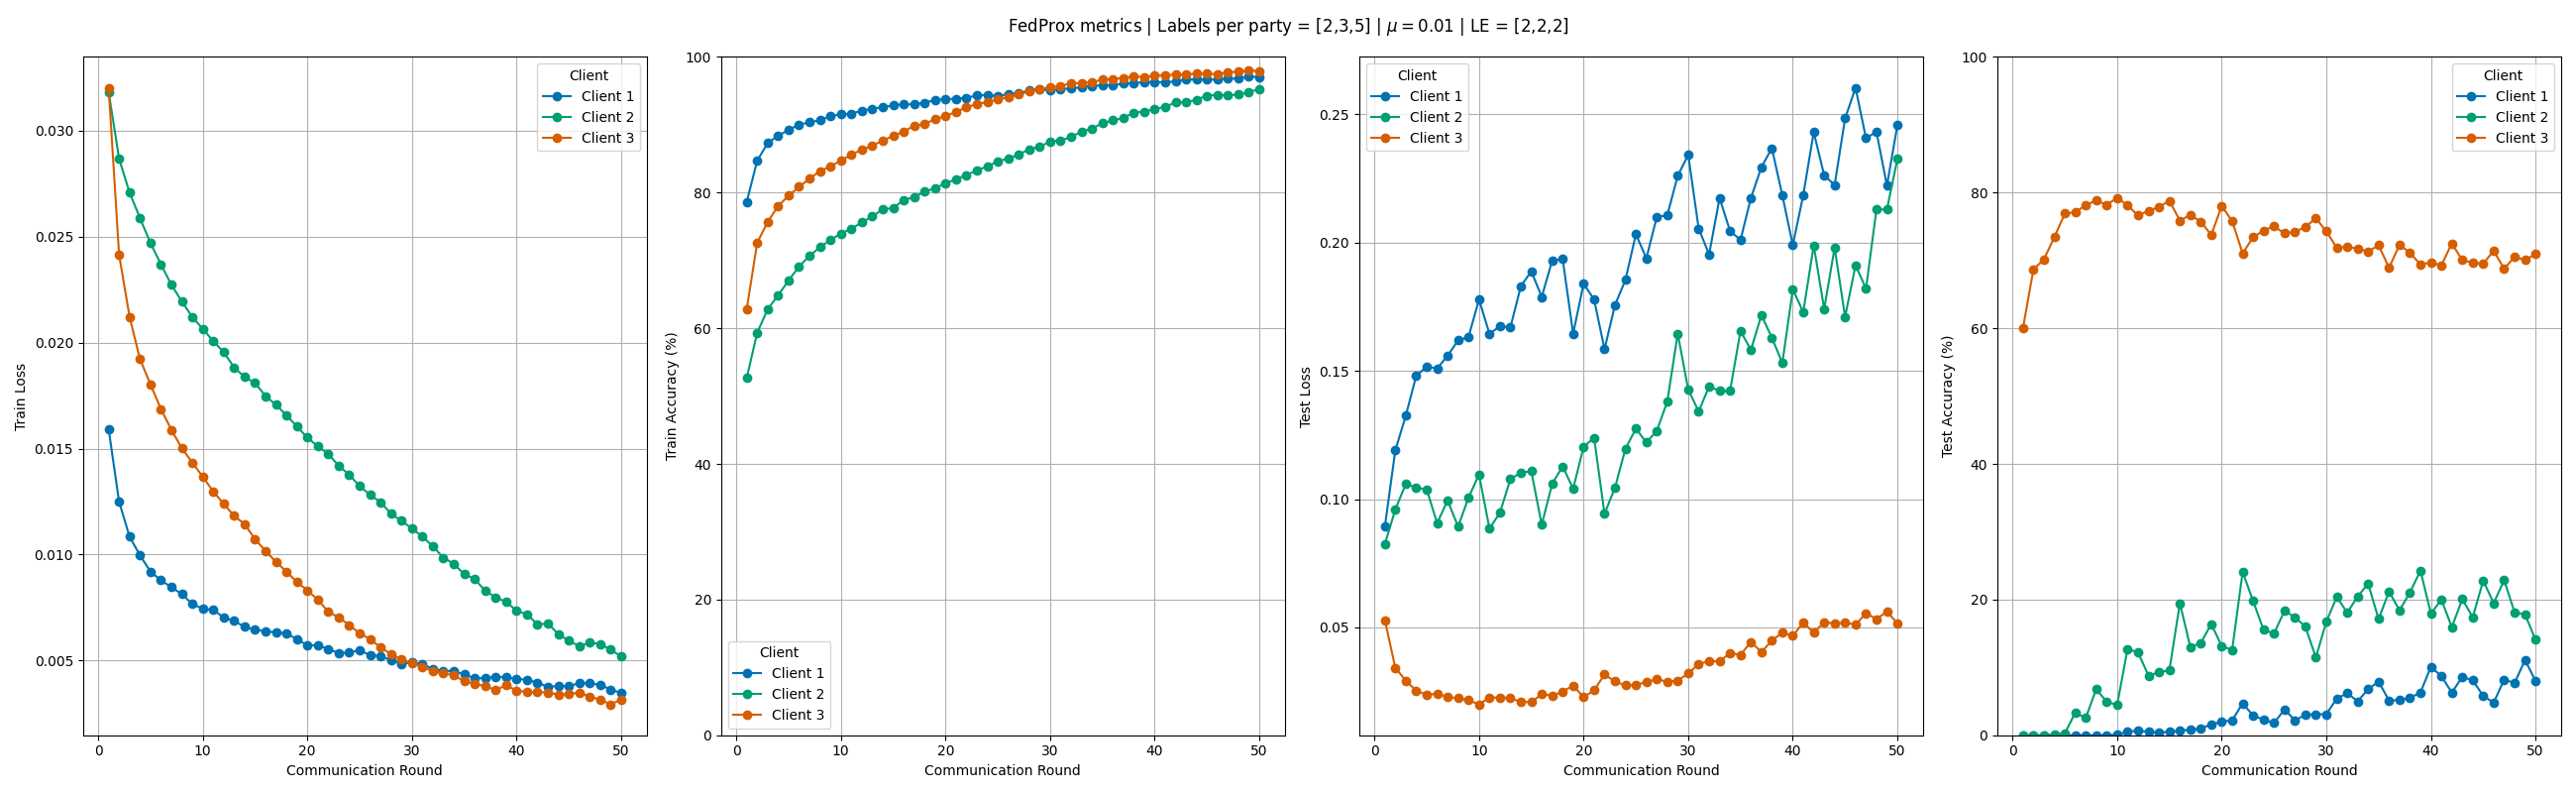
\includegraphics[width=0.8\textwidth]{figures/2-Federated_Learning/FedProx_LabelsPerParty_mu_0.01.png}
  \caption{Local metrics for FedProx, $\mu = 0.01$, label distribution skew with a disjoint partition of $[2,3,5]$.}
  \label{fig:FedProx_LabelsPerParty_Mu_0.01}
\end{figure}

As we see from Figure \ref{fig:FedProx_LabelsPerParty_Mu_0.01}, a better performance has been achieved compared with the same setting using FedAvg, although the improvement is modest and mainly for client 1, whose previous accuracy was near 0 since only holds 2 labels.

\begin{figure}[H]
  \centering
  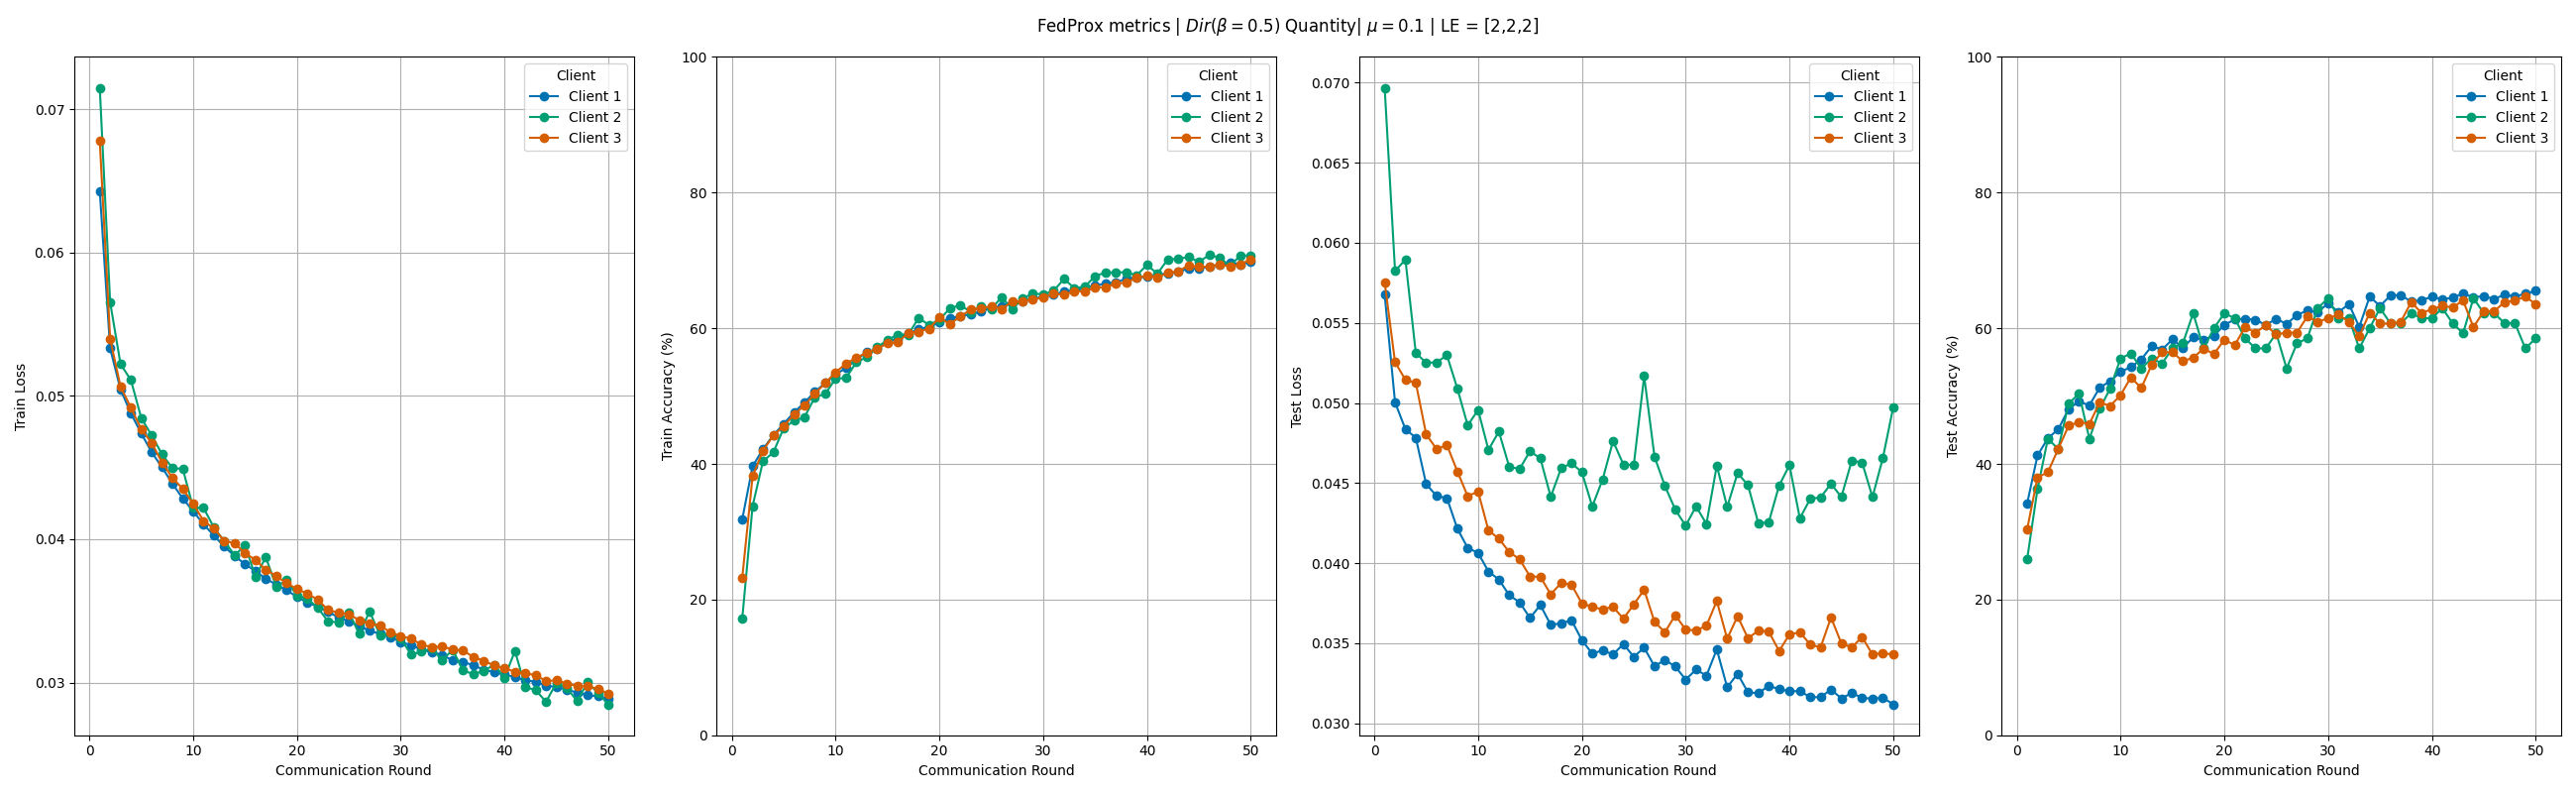
\includegraphics[width=0.8\textwidth]{figures/2-Federated_Learning/FedProx_QuantitySkew_Dir_05_Mu_0.1.png}
  \caption{Local metrics for FedProx, $\mu = 0.1$, label quantity skew using $Dir(\boldsymbol{\beta})$, $\boldsymbol{\beta} = (0.5,0.5,0.5)$.}
  \label{fig:FedProx_LabelsQuantitySkew_Dir_05_Mu_0.1}
\end{figure}

\begin{figure}[H]
  \centering
  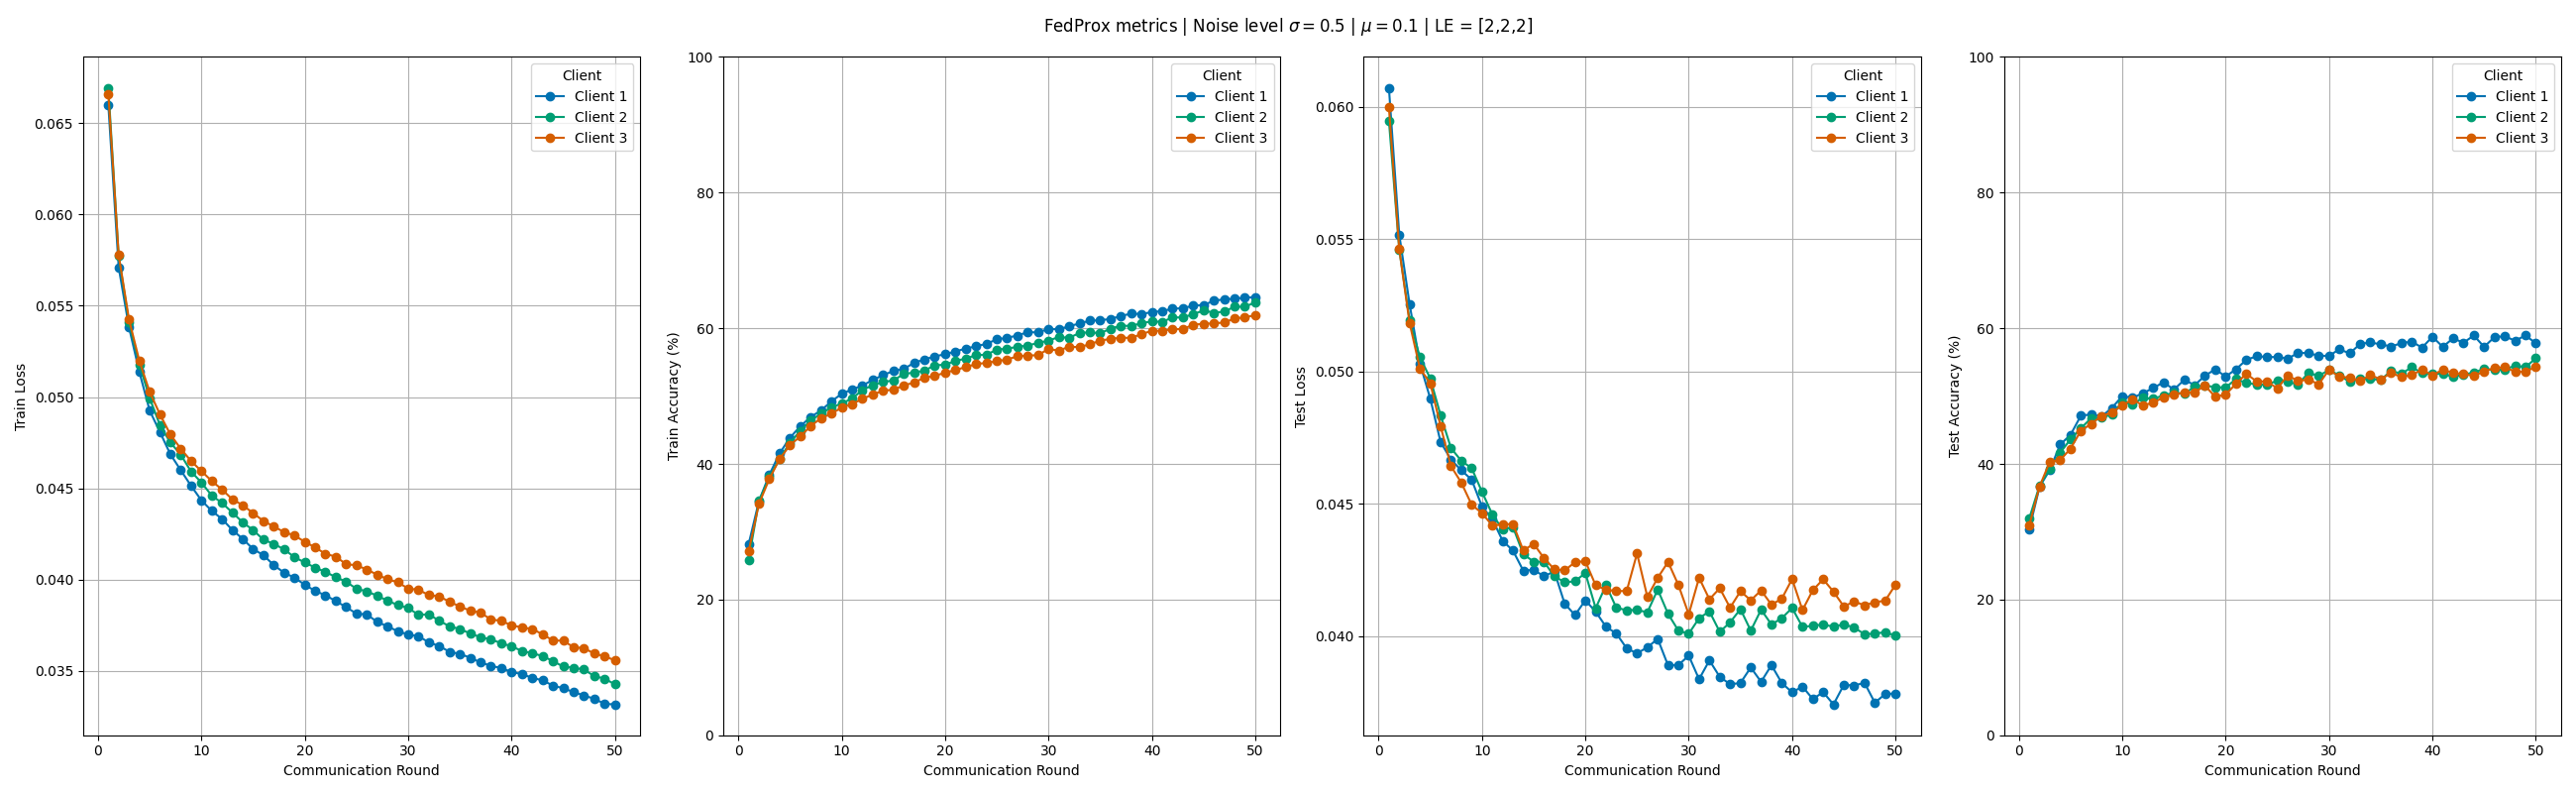
\includegraphics[width=0.8\textwidth]{figures/2-Federated_Learning/FedProx_NoiseLevel_Mu_0.1.png}
  \caption{Local metrics for FedProx, $\mu = 0.1$, feature distribution skew using a noise level of $\sigma = 0.5$.}
  \label{fig:FedProx_Noise_Dir_05_Mu_0.1}
\end{figure}

In Figure \ref{fig:FedProx_LabelsQuantitySkew_Dir_05_Mu_0.1} all clients have a better test accuracy compared with the FedAvg experiment (in the same setting). For the feature skew, we see that the performance seen in Figure \ref{fig:FedProx_Noise_Dir_05_Mu_0.1} is similar to the one in \ref{fig:FedAvg_Noise_level}.

\begin{table}[h]
    \centering
    \begin{tabular}{lccccc}
        \toprule
        & IID & Label Skew Dir(0.5) & Quantity Skew Dir(0.5) & Labels per Party & Noise $\sigma = 0.5$ \\
        \midrule
        FedAvg & \textbf{0.6427} & 0.4335 & 0.6192 & 0.3934 & 0.5933 \\
        FedProx Mu 0.001 & 0.6425 & 0.4466 & 0.6309 & 0.4034 & 0.5961 \\
        FedProx Mu 0.01 & 0.6356 & \textbf{0.4505} & \textbf{0.6494} & \textbf{0.4435} & \textbf{0.5979} \\
        FedProx Mu 0.1 & 0.6363 & 0.4347 & 0.6396 & 0.4226 & 0.5906 \\
        FedProx Mu 1 & 0.4443 & 0.4034 & 0.4238 & 0.3437 & 0.4375 \\
        \bottomrule
    \end{tabular}
    \caption{Top global test accuracy obtained in FedAvg and FedProx under the same settings for different values of $\mu$.}
    \label{tab:accuracy}
\end{table}

\section{FedNova}

This algorithm was first introduced in \cite*{wang2020}, in order to study its main contributions we are changing the original notation of \textit{FedAvg}. We have seen that the client updates its model at round $t$ starting with a shared, global model $\omega_g^t$. Then, it applies SGD with its local data for a fixed number of epochs E.
We recall that, for each epoch, and for each batch $\mathbf{b} = \{\mathbf{x}, y\} \in \mathcal{B} \subset D^i$, the i-th client performs $\omega_i^t = \omega_i^t - \eta \nabla l_i(\omega_i^t, \mathbf{b})$. After the round, the client will have a locally updated model $\omega_i^{t+1}$. After all the clients have updated their models, it aggregates them following the formula: $\omega_g^{t+1} = \sum_{k \in S_t} \frac{|D^k|}{\sum_{k\in S_t} |D^k|} w_k^{t+1}$.
We can now consider the difference between the global client's starting model $\omega_g^t$ and its locally updated model $\omega_i^{t+1}$, we will denote $\Delta \omega_i^t \coloneqq \omega_g^t - \omega_i^{t+1}$, the difference between the global model at time $t$ and the local model of client $i$ at time $t+1$.
The server would then collect $\Delta \omega_k^t$ $\forall k \in \{1,\dots, N\}$ and update the global model. For example, in \textit{FedAvg}: $\omega_g^{t+1} = \omega_g^t + \sum_{k \in S_t} \alpha_k \Delta \omega_k^t = \omega_g^t - \sum_{k \in S_t} \alpha_k \eta \sum_{j=1}^{\tau_k} g_k(\omega_k^{t, j})$ where $\alpha_k = \frac{|D^k|}{\sum_{k\in S_t} |D^k|}$, $\tau_k = \lfloor \frac{E_k |D^k|}{B} \rfloor$ with $B$ being the mini-batch size and $E_k$ the local number of epochs of client $k$, $\omega_k^{t,j}$ is the client k's model after the j-th SGD update at time $t$, $\eta$ is the learning rate (same for all clients) and $g_k$ is the stochastic gradient over a mini-batch $\mathbf{b} \in \mathcal{B}$.\\
As stated in \cite*{wang2020}, different $E_k$ across clients and rounds means that $FedAvg$ algorithm converges to a surrogate objective instead of $F(\omega)$ from (\ref{eqn:objective}).
This algorithm considers that different parties compute a different number of local steps ($\tau_k$) because of computation constraints or different sizes of local datasets. When $\tau_{k} > \tau_{k'}$, client $k$ will have a major influence over the global update rule compared to client $k'$. That's why the authors proposed to normalize and scale the local updates according to the number of local steps.

\begin{figure}[H]
  \centering
  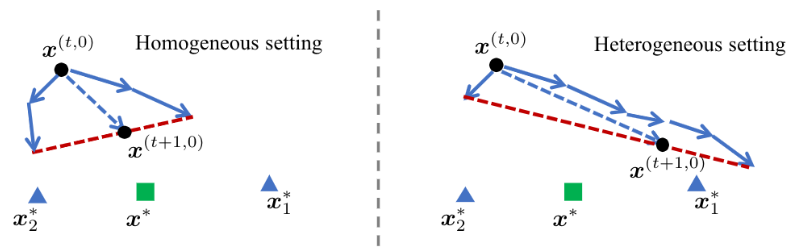
\includegraphics[width=0.8\textwidth]{figures/2-Federated_Learning/FedNova_Normalization_model_drift.png}
  \caption{Model updates in the parameter space. Green squares and blue triangles denote the minima of global and local objectives, respectively. Source: \cite{wang2020}}
  \label{fig:FedNova_Normalization_model_drif}
\end{figure}

\begin{algorithm}[H]
  \label{alg:FedNova}
  \caption{FedNova}
  \begin{algorithmic}[1]
    \Require{local datasets $D^i$ $\forall i \in \{1,\dots, N\}$, number of parties $N$, number of communication rounds $T$, number of local epochs $E$, learning rate $\eta$, local mini-batch size $B$.}
    \Ensure{global model $\omega^T_g$.}
    \Statex
    \Procedure{Server execution}{}
    \State Initialize $\omega_g^0$
    \For {round $t = 1,\dots, T$}
      \State $S_t$  (Selection of clients)
      \For {client $k \in S_t$ \textbf{in parallel}}
        \State $\Delta \omega_k^{t}, \tau_k \gets ClientUpdate(k, \omega_g^t)$
      \EndFor
      \State $n \gets \sum_{k \in S_t} |D^k|$
      \State $\omega_g^{t+1} \gets \omega_g^t - \eta \frac{\sum_{k \in S_t} |D^k| \tau_k}{n} \sum_{k \in S_t} \frac{|D^k| \Delta \omega_k^t}{\tau_k n}$
    \EndFor
    \EndProcedure

    \Procedure{$ClientUpdate(k, \omega_g^t)$}{}
    \State $\omega_k^t \gets \omega_g^t$
    \State $\tau_k \gets 0$
    \State $\mathcal{B} \gets$ Batches of $D^k$ of size $B$
    \For {local epoch $i=1,\dots,E$}
      \For {batch $\mathbf{b} \in \mathcal{B}$}
        \State $\omega_k^t \gets \omega_k^t - \eta \nabla l(\omega_k^t; \mathbf{b})$
        \State $\tau_k \gets \tau_k + 1$
      \EndFor
    \EndFor
    \State $\Delta \omega_k^t \gets \omega_g^t - \omega_k^t$
    \State return $\Delta \omega_k^t$, $\tau_k$  to the server.
    \EndProcedure
  \end{algorithmic}
\end{algorithm}

For the next experiments, the same data distribution and initial weights will be used for both FedAvg and FedNova, starting with an IID setting:


\begin{figure}[H]
  \centering
  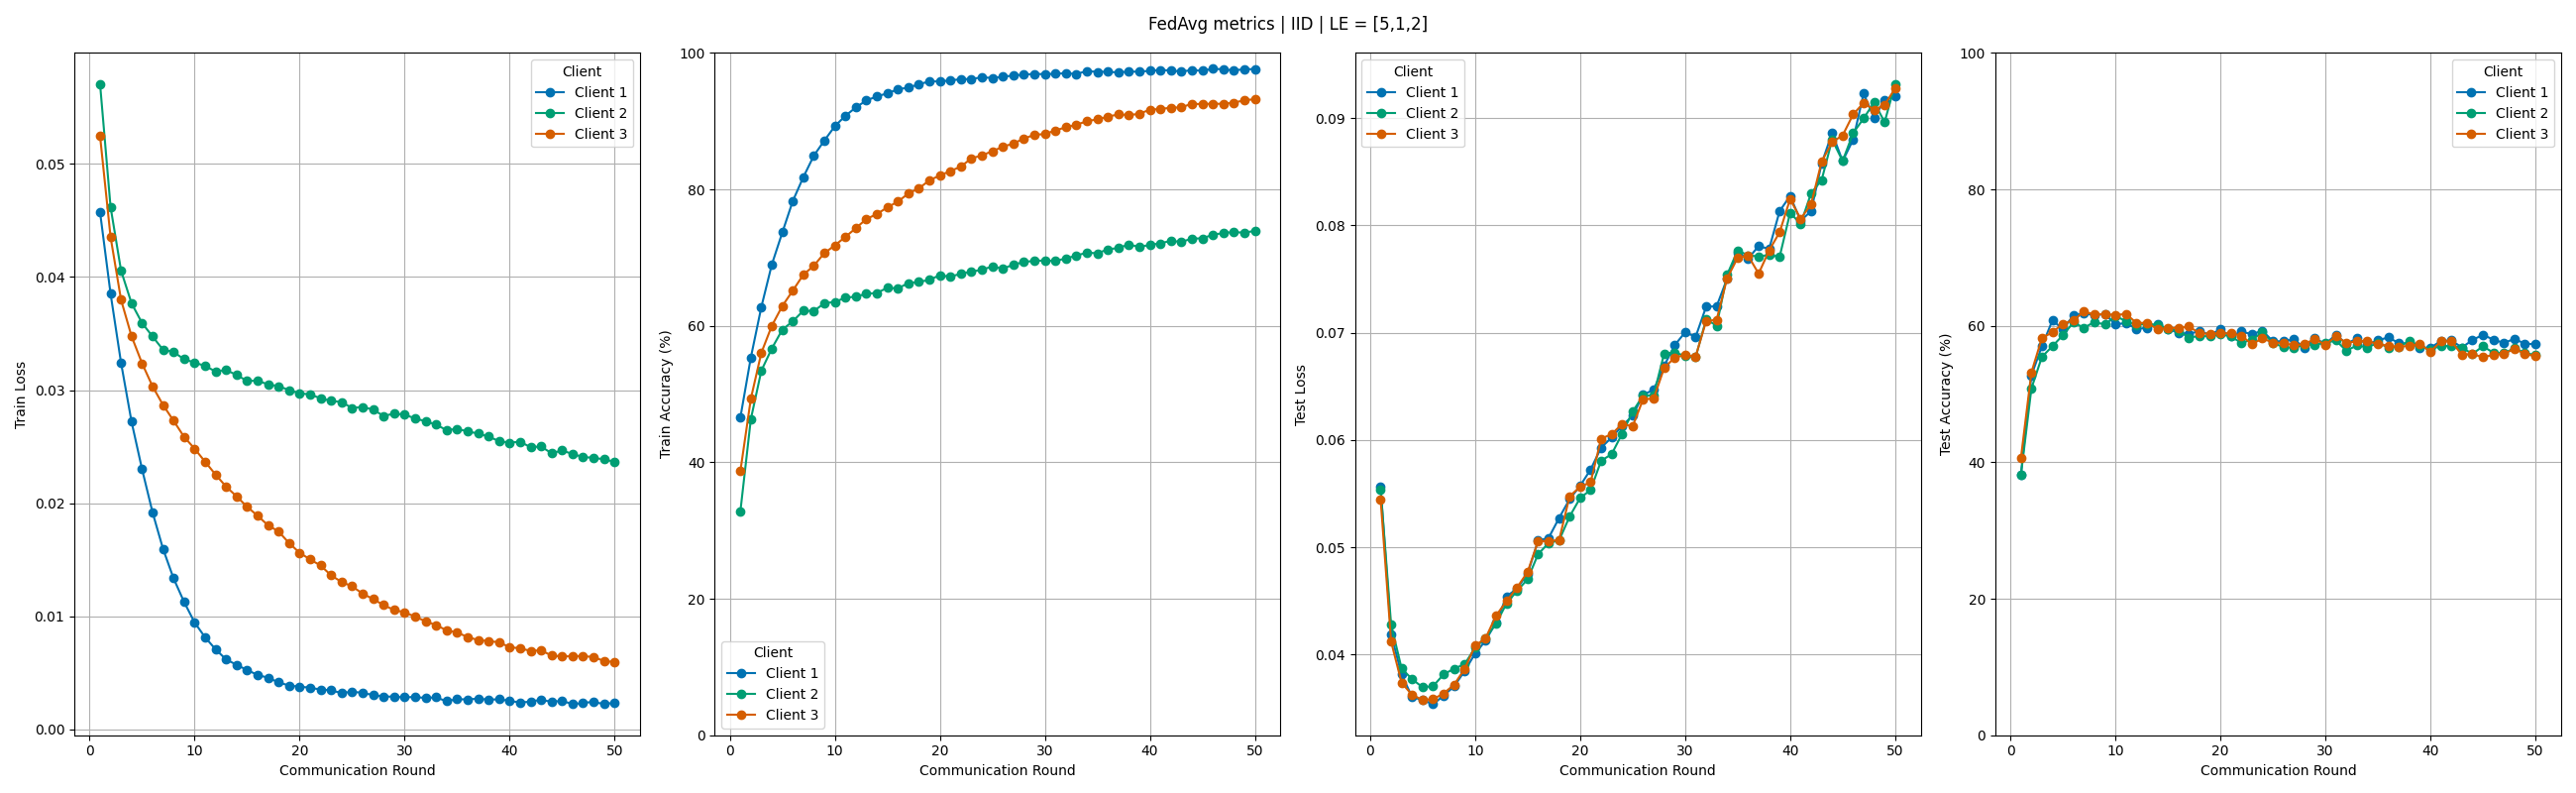
\includegraphics[width=0.9\textwidth]{figures/2-Federated_Learning/FedAvg_IID_LE_512.png}
  \caption{Local metrics for FedAvg on a IID setting with local epochs [5,1,2].}
  \label{fig:FedAvg_IID_LE_512}
\end{figure}


\begin{figure}[H]
  \centering
  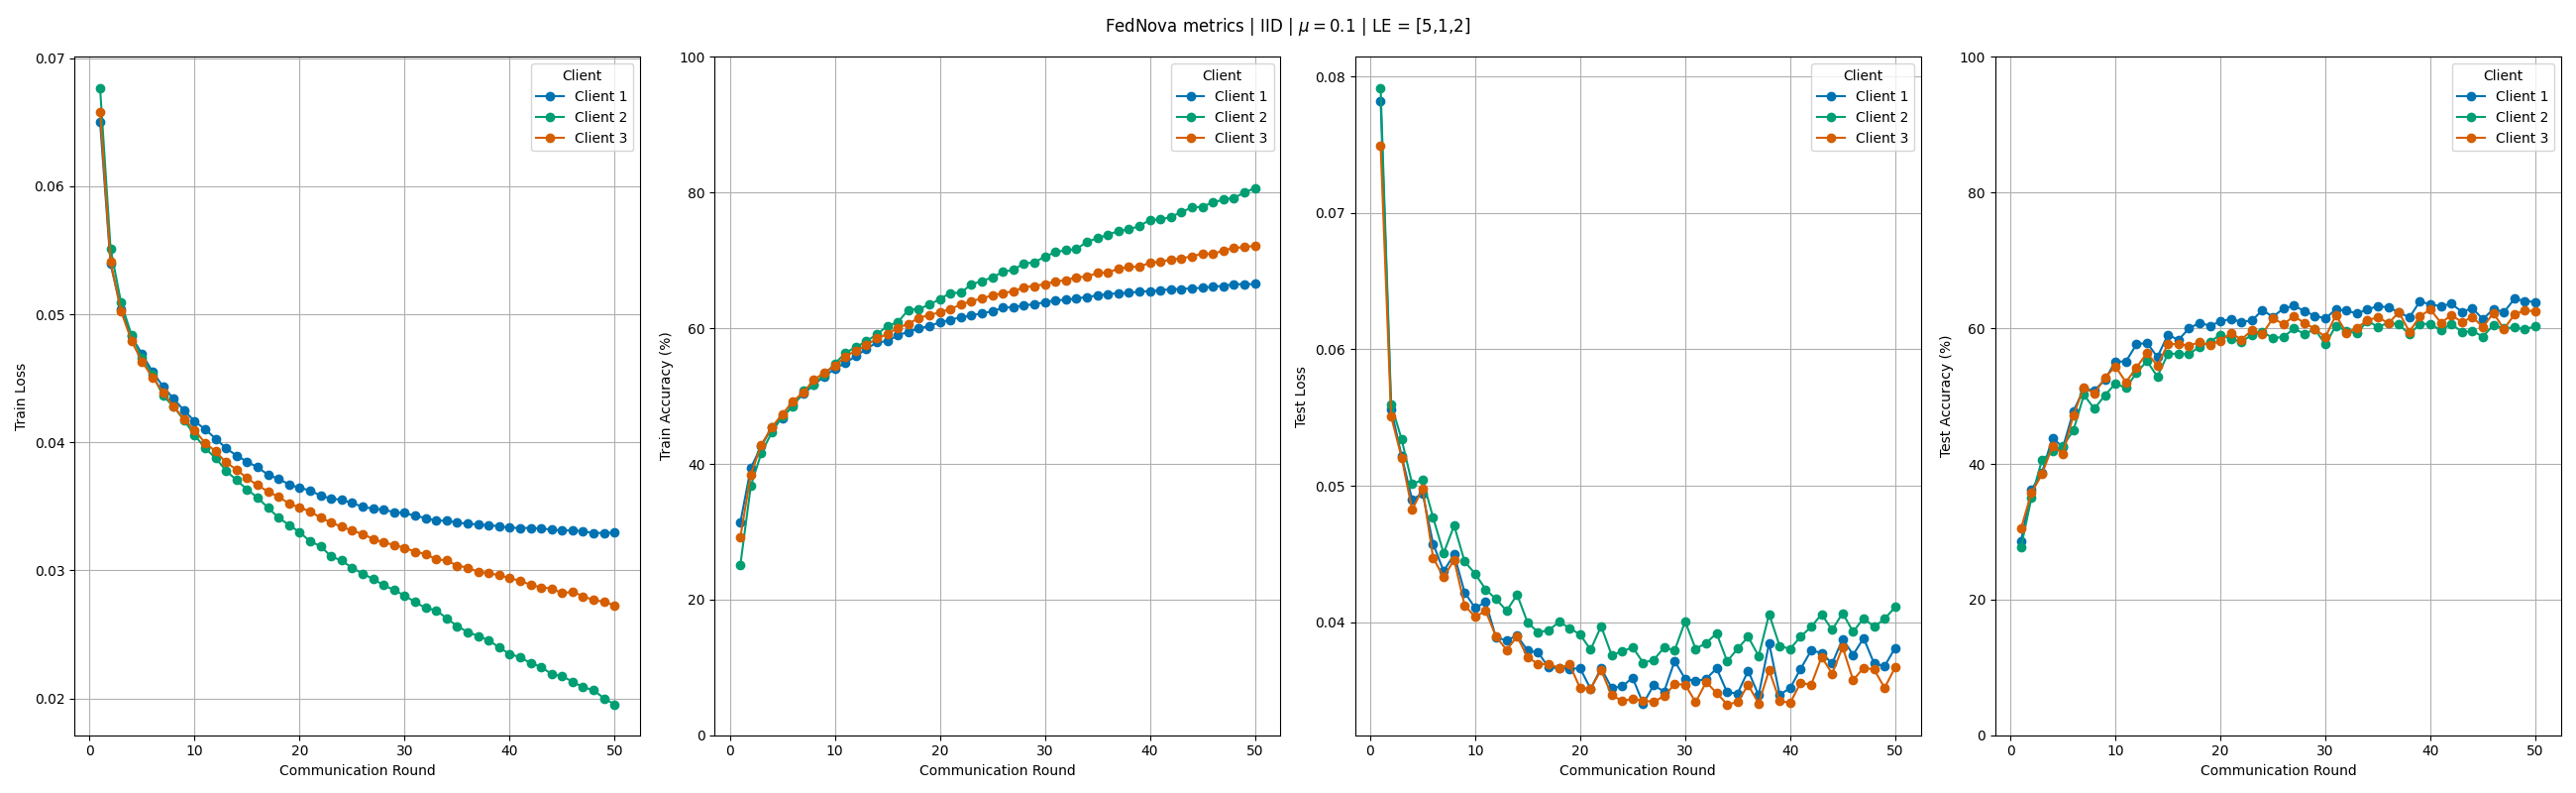
\includegraphics[width=0.9\textwidth]{figures/2-Federated_Learning/FedNova_IID_LE_512.png}
  \caption{Local metrics for FedNova using proximal term with $\mu=0.1$ on a IID setting and local epochs [5,1,2].}
  \label{fig:FedNova_IID_LE_512}
\end{figure}

We have used FedNova with a local loss modified as explained with FedProx, since both approach are compatible. We see a slightly improvement with FedNova compared to FedAvg in a IID setting. Note that the first client performs 5 local epochs, the second client only 1 epoch and the third client 2 epochs (assuming some kind of computational or communication constraint). However, for a label skew setting using the Dirichlet distribution, Figures \ref{fig:FedAvg_NonDirichlet_LE_512} and \ref{fig:FedNova_NonDirichlet_LE_512}, the client with more epochs (client 1) got lower test accuracy compared to the others clients, since as the client's data is scarce (see Figure \ref{fig:label_distribution_skew_Dirichlet} for each client's distribution). More local epochs doesn't mean that the client will perform better on its own local data, since the aggregation step changes all its model weights favoring the clients with more data.


\begin{figure}[H]
  \centering
  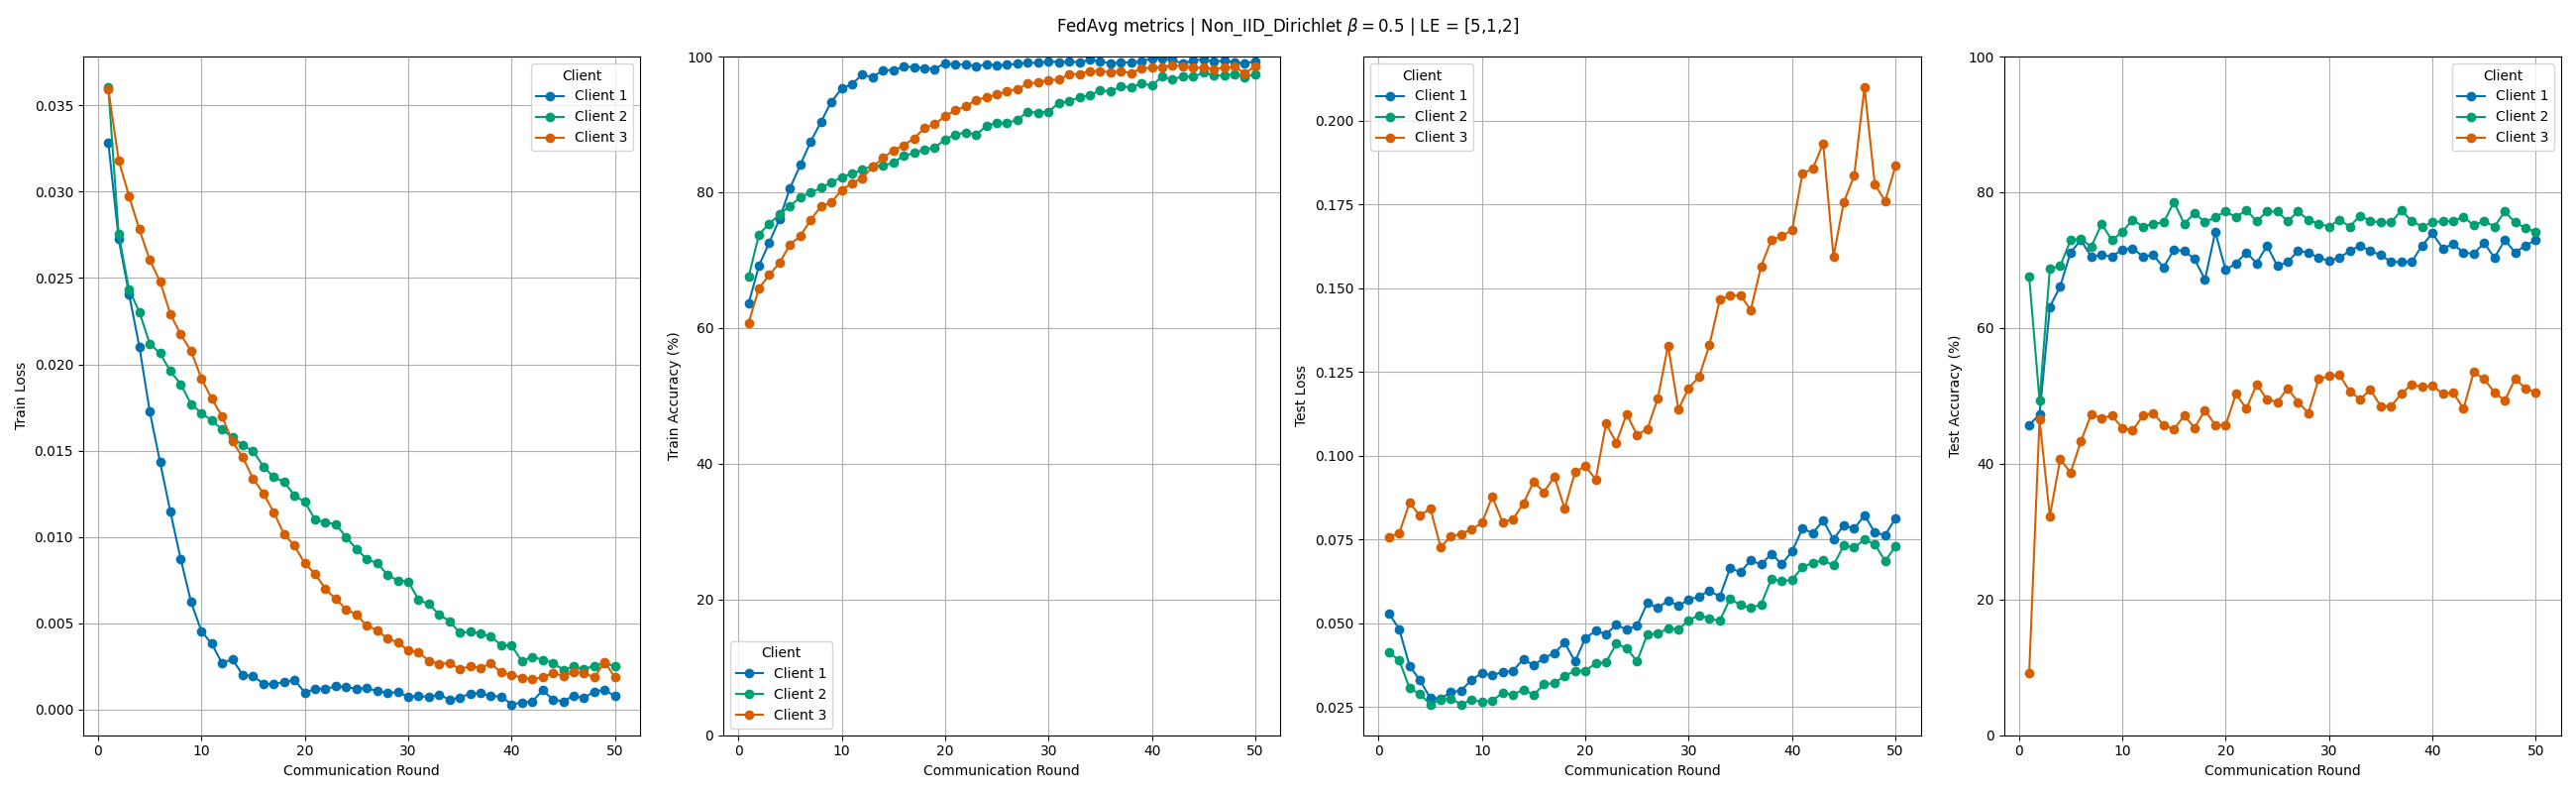
\includegraphics[width=0.9\textwidth]{figures/2-Federated_Learning/FedAvg_NonDirichlet_LE_512.png}
  \caption{Local metrics for FedAvg on a Non-IID label skew using $Dir(\boldsymbol{\beta})$, $\boldsymbol{\beta}=(0.5, 0.5, 0.5)$ setting with local epochs [5,1,2].}
  \label{fig:FedAvg_NonDirichlet_LE_512}
\end{figure}


\begin{figure}[H]
  \centering
  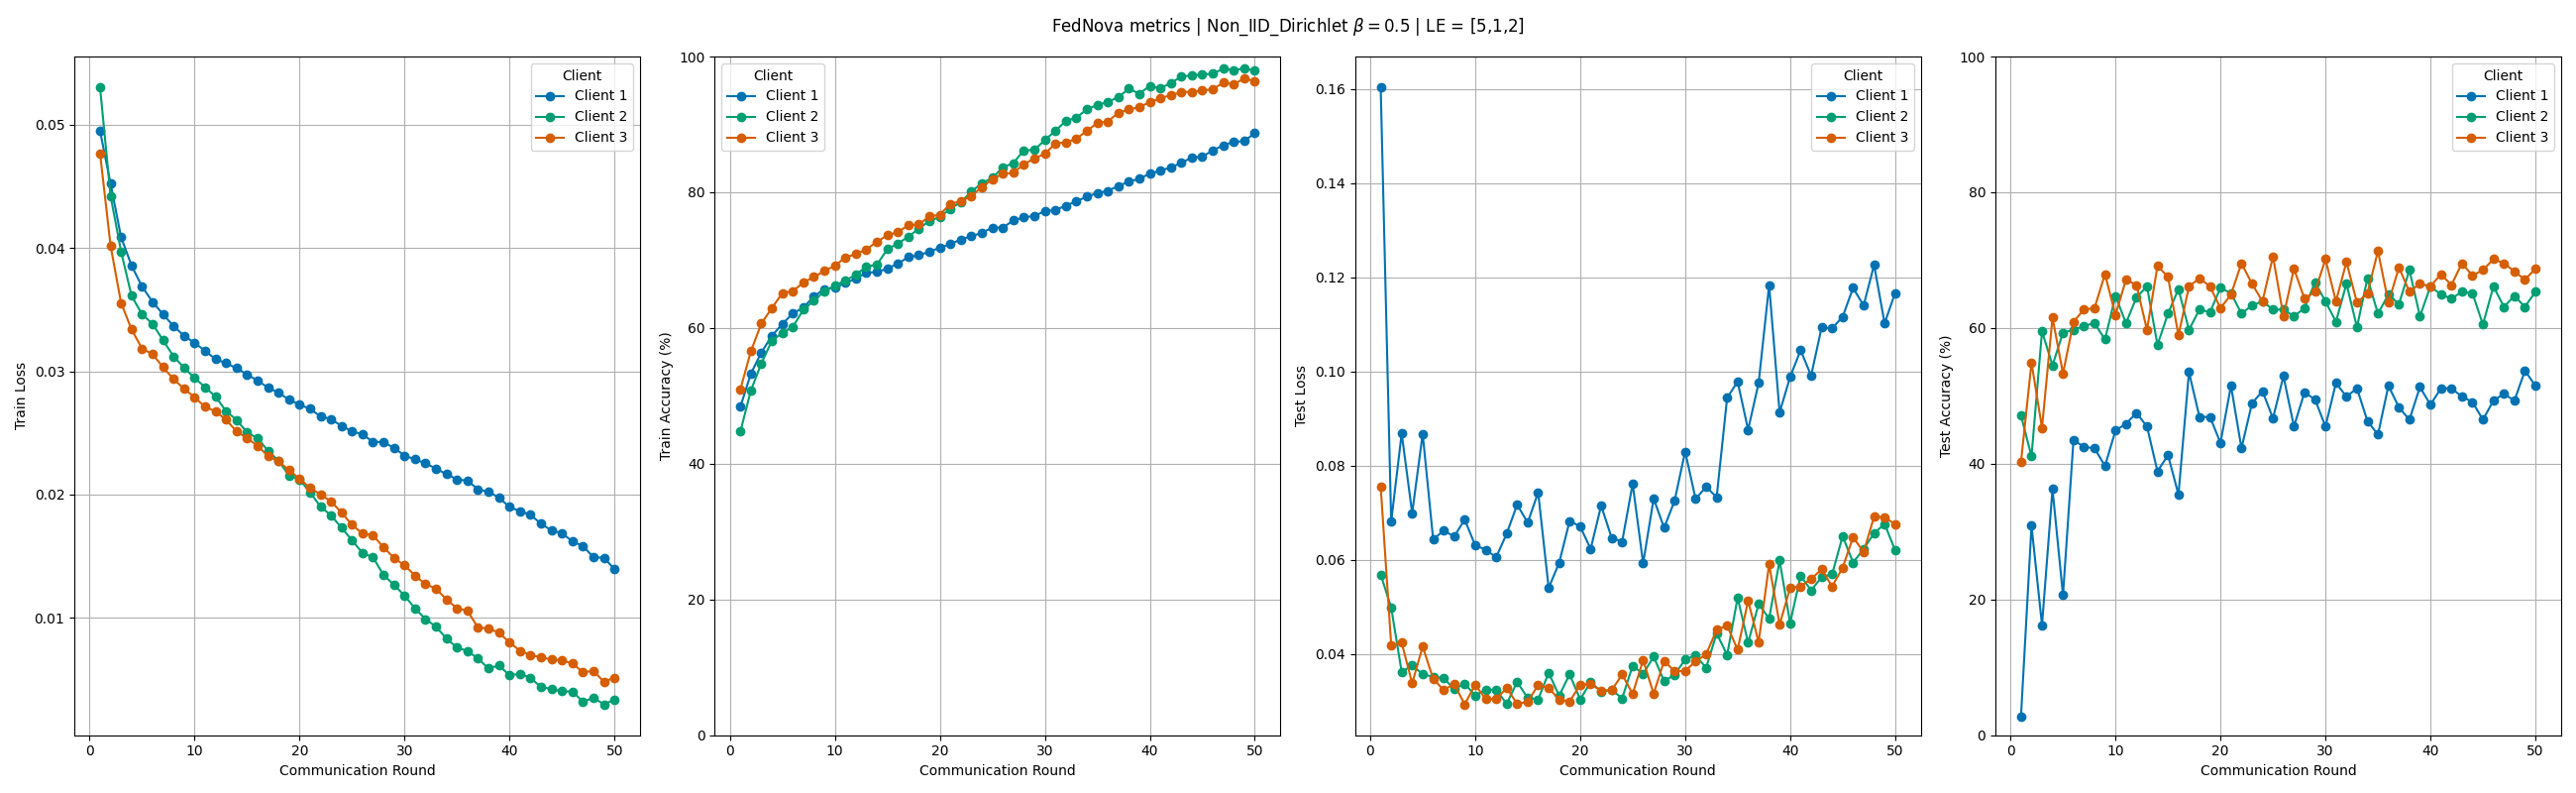
\includegraphics[width=0.9\textwidth]{figures/2-Federated_Learning/FedNova_NonDirichlet_LE_512.png}
  \caption{Local metrics for FedNova using proximal term with $\mu=0.1$ on a Non-IID setting label skew using $Dir(\boldsymbol{\beta})$, $\boldsymbol{\beta}=(0.5, 0.5, 0.5)$ and local epochs [5,1,2].}
  \label{fig:FedNova_NonDirichlet_LE_512}
\end{figure}

We see in this case that FedNova doesn't perform better than FedAvg, although we will compare the model's accuracy later with the global dataset. This is something that some articles have already commented: FedNova doesn't perform better than other approaches or even FedAvg in some Non-IID scenarios \cite{li2021}.
In fact, in the next experiment we can see that using FedNova performs worse than FedAvg for both clients 1 and 3, where client 1 holds two labels and client 3 holds 3 labels. From the previous expriment we have seen that this setting is the one that hurts the model accuracy the most.
\begin{figure}[H]
  \centering
  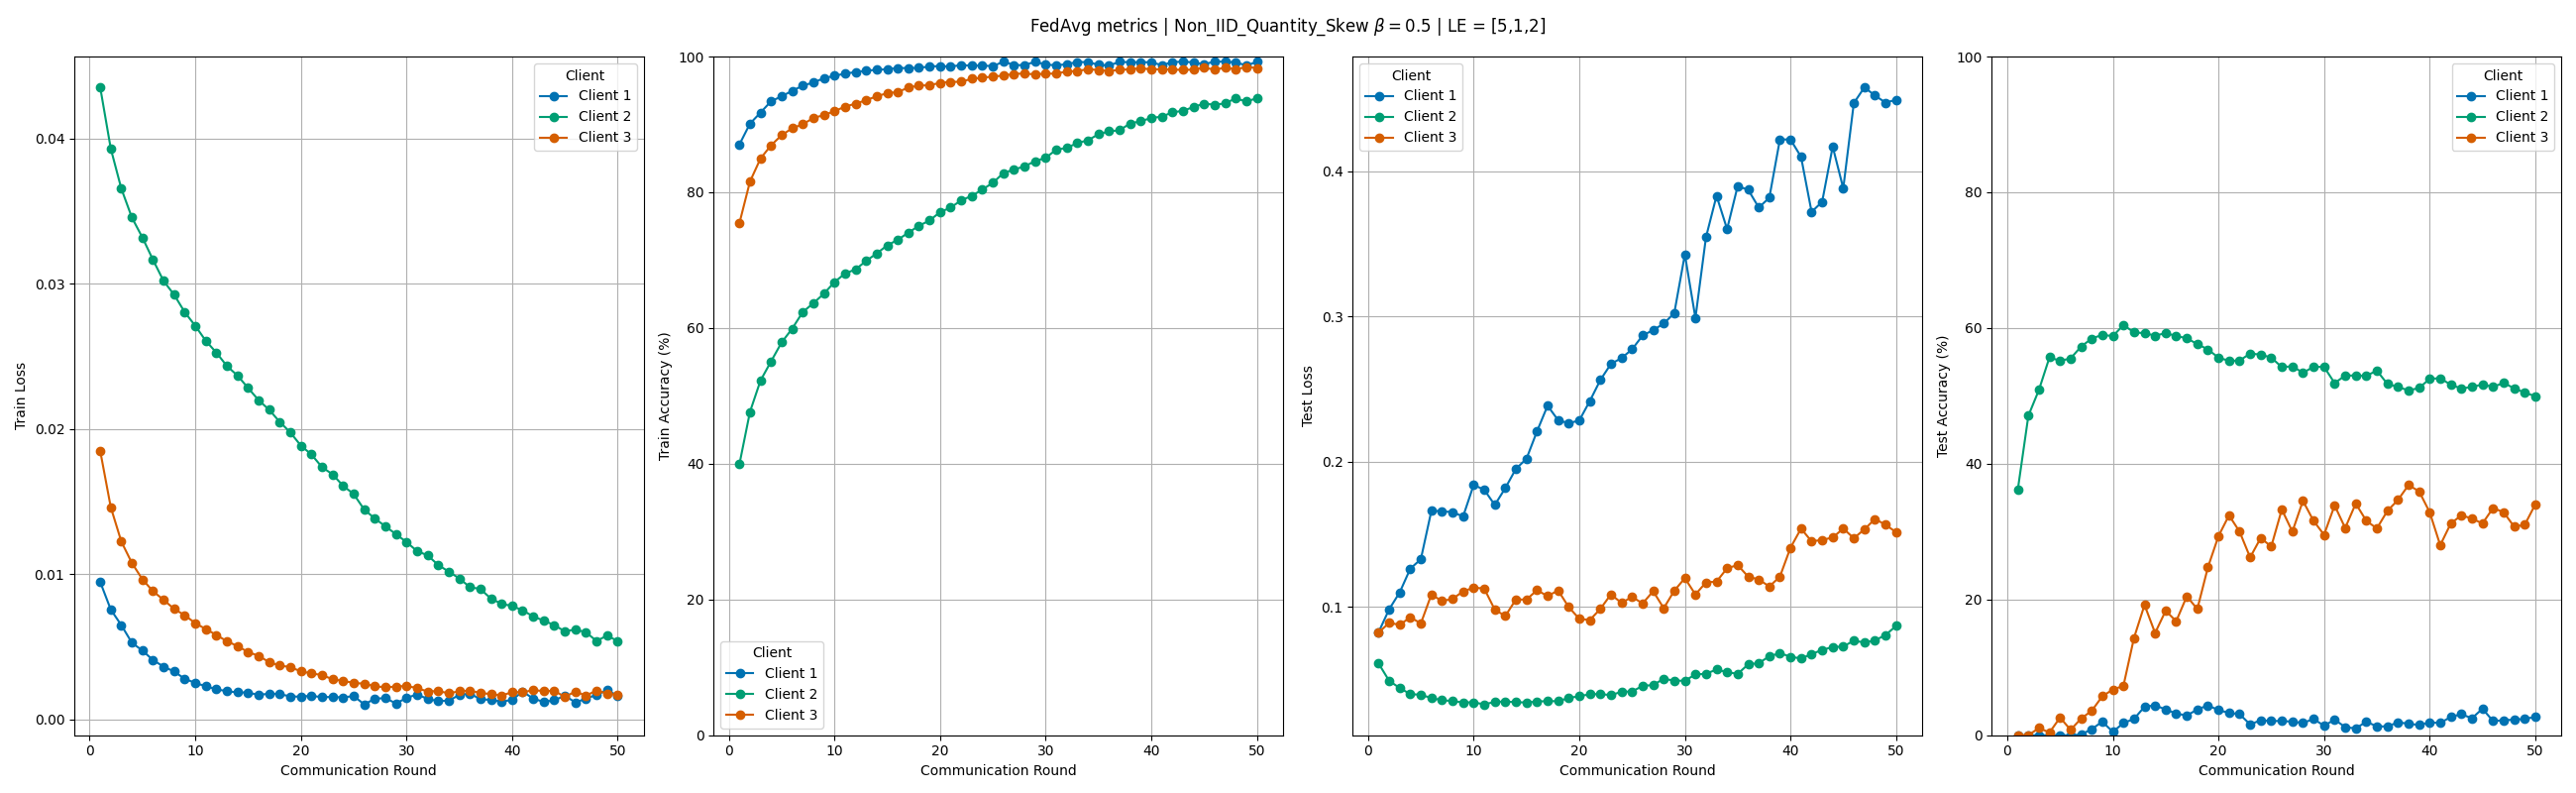
\includegraphics[width=0.9\textwidth]{figures/2-Federated_Learning/FedAvg_QuantityBased_Labels_253_LE_512.png}
  \caption{Local metrics for FedAvg  on a Non-IID setting Quantity-based (labels per party = [2,5,3]) and local epochs [5,1,2].}
  \label{fig:FedAvg_QuantityBased_LabelsPerParty_253_LE_512}
\end{figure}


\begin{figure}[H]
  \centering
  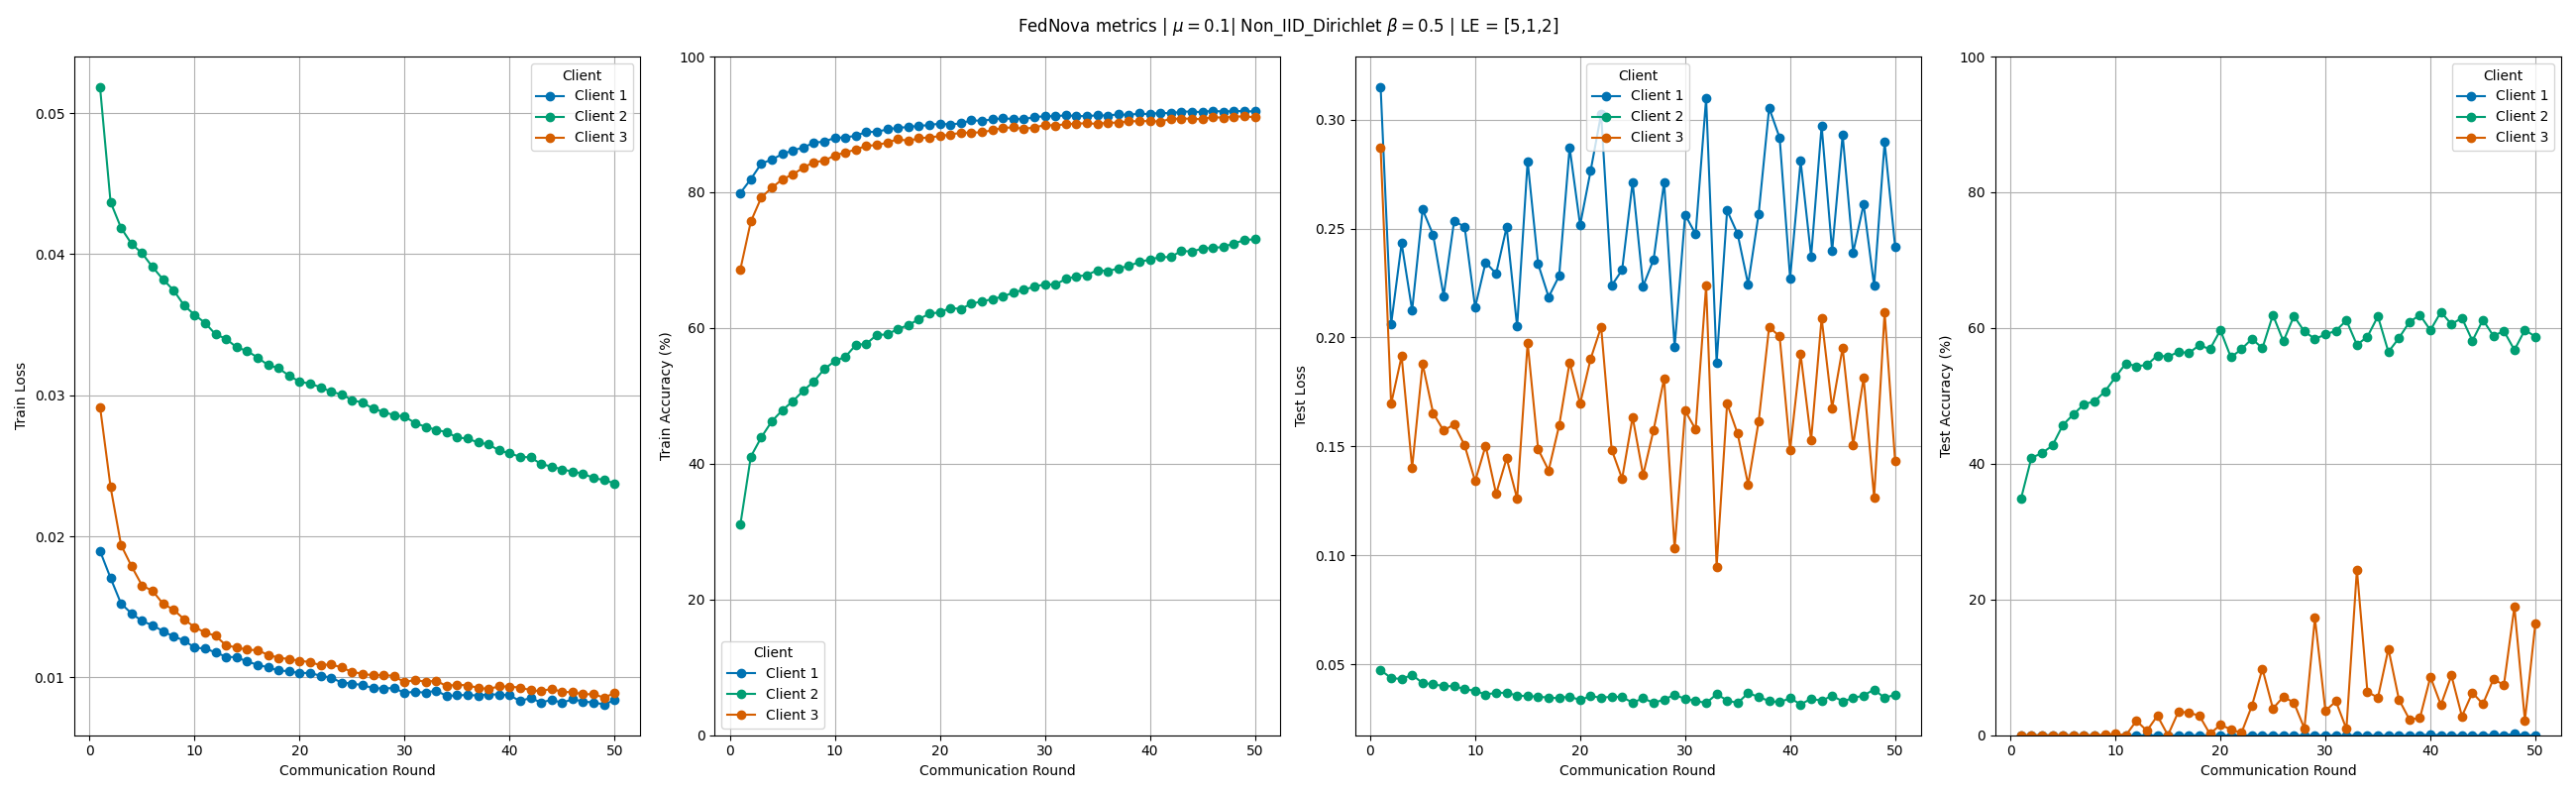
\includegraphics[width=0.9\textwidth]{figures/2-Federated_Learning/FedNova_QuantityBased_Labels_253_LE_512.png}
  \caption{Local metrics for FedNova using a proximal term with $\mu=0.1$ on a Non-IID setting Quantity-based (labels per party = [2,5,3]) and local epochs [5,1,2].}
  \label{fig:FedNova_QuantityBased_LabelsPerParty_253_LE_512}
\end{figure}

In Fugures \ref{fig:FedAvg_QuantitySkew_LE_512} and \ref{fig:FedNova_QuantitySkew_LE_512}, FedNova has slightly better results for clients 1 and 2 but client 3 doesn't converge at all, making FedAvg a more stable approach in this case.

\begin{figure}[H]
  \centering
  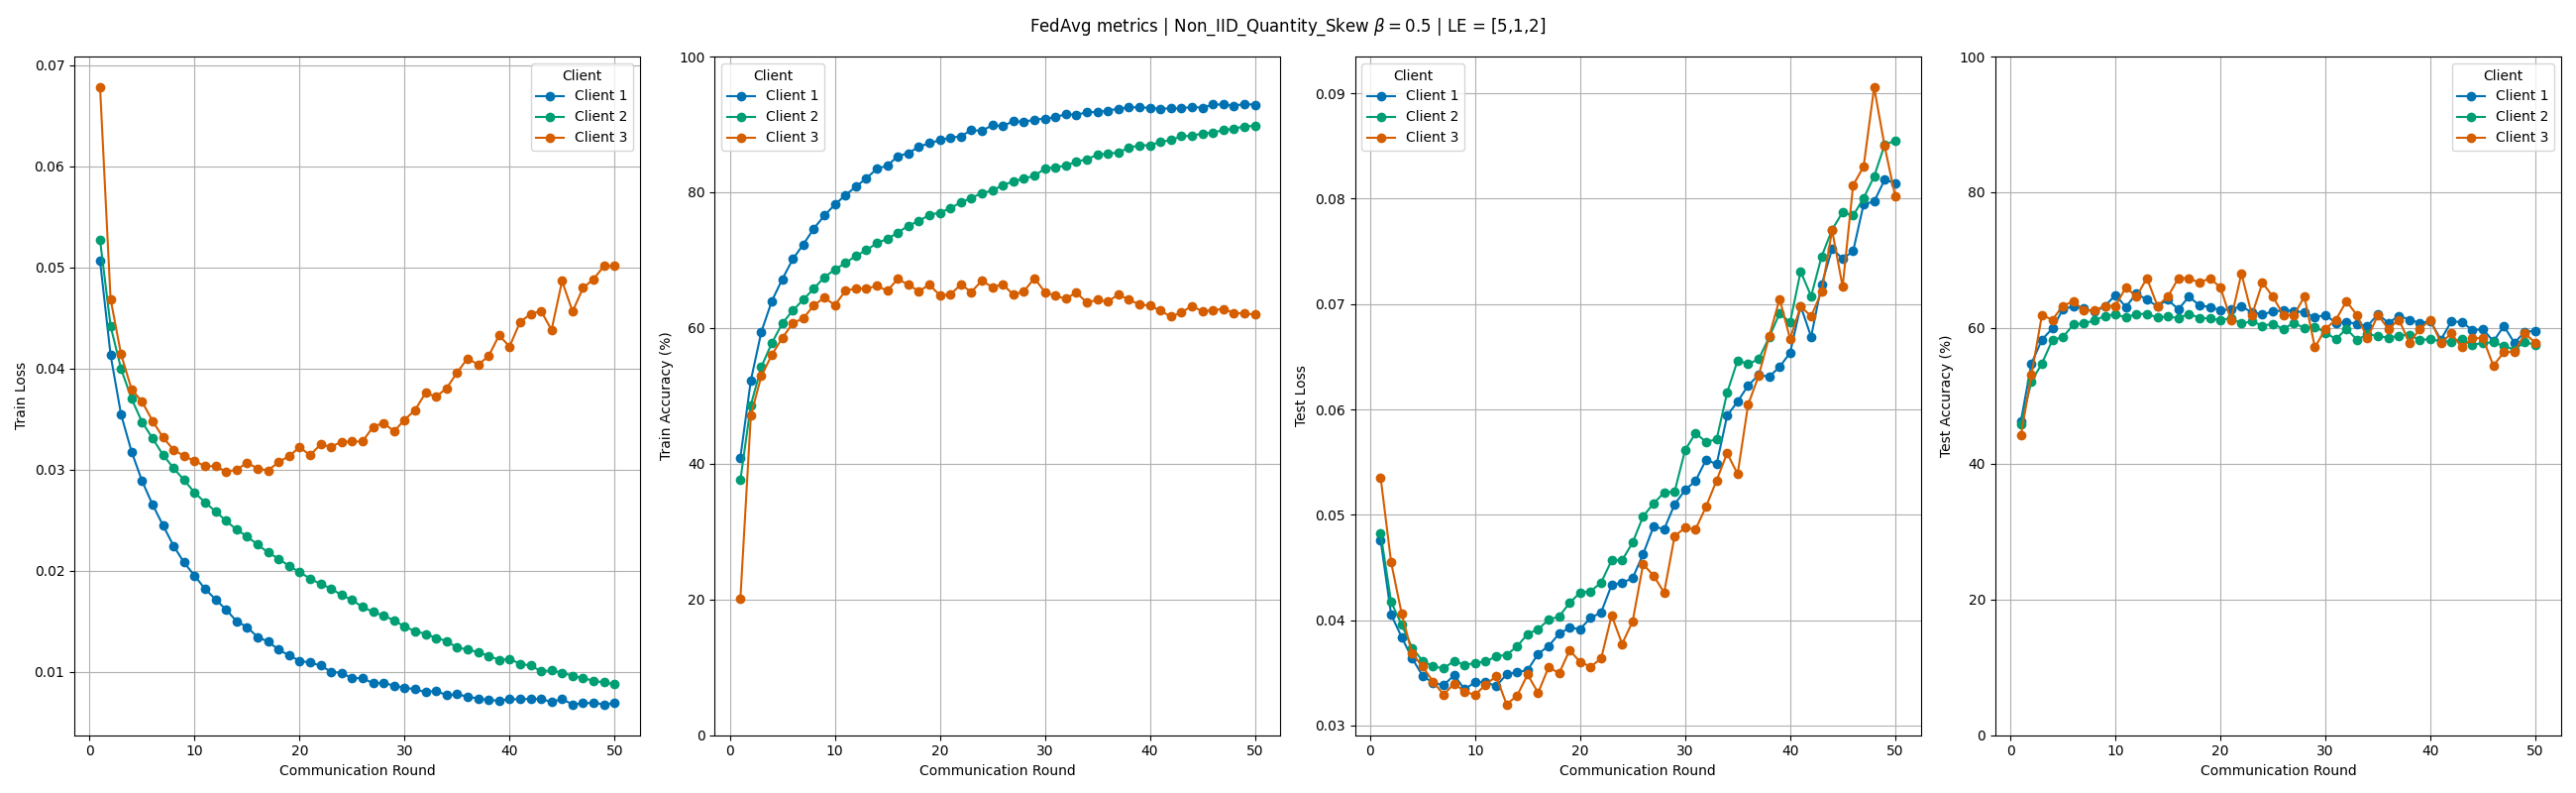
\includegraphics[width=0.9\textwidth]{figures/2-Federated_Learning/FedAvg_QuantitySkew_LE_512.png}
  \caption{Local metrics for FedAvg  on a Non-IID Quantity Skew setting using $Dir(\boldsymbol{\beta})$, $\boldsymbol{\beta}=(0.5, 0.5, 0.5)$ and local epochs [5,1,2].}
  \label{fig:FedAvg_QuantitySkew_LE_512}
\end{figure}


\begin{figure}[H]
  \centering
  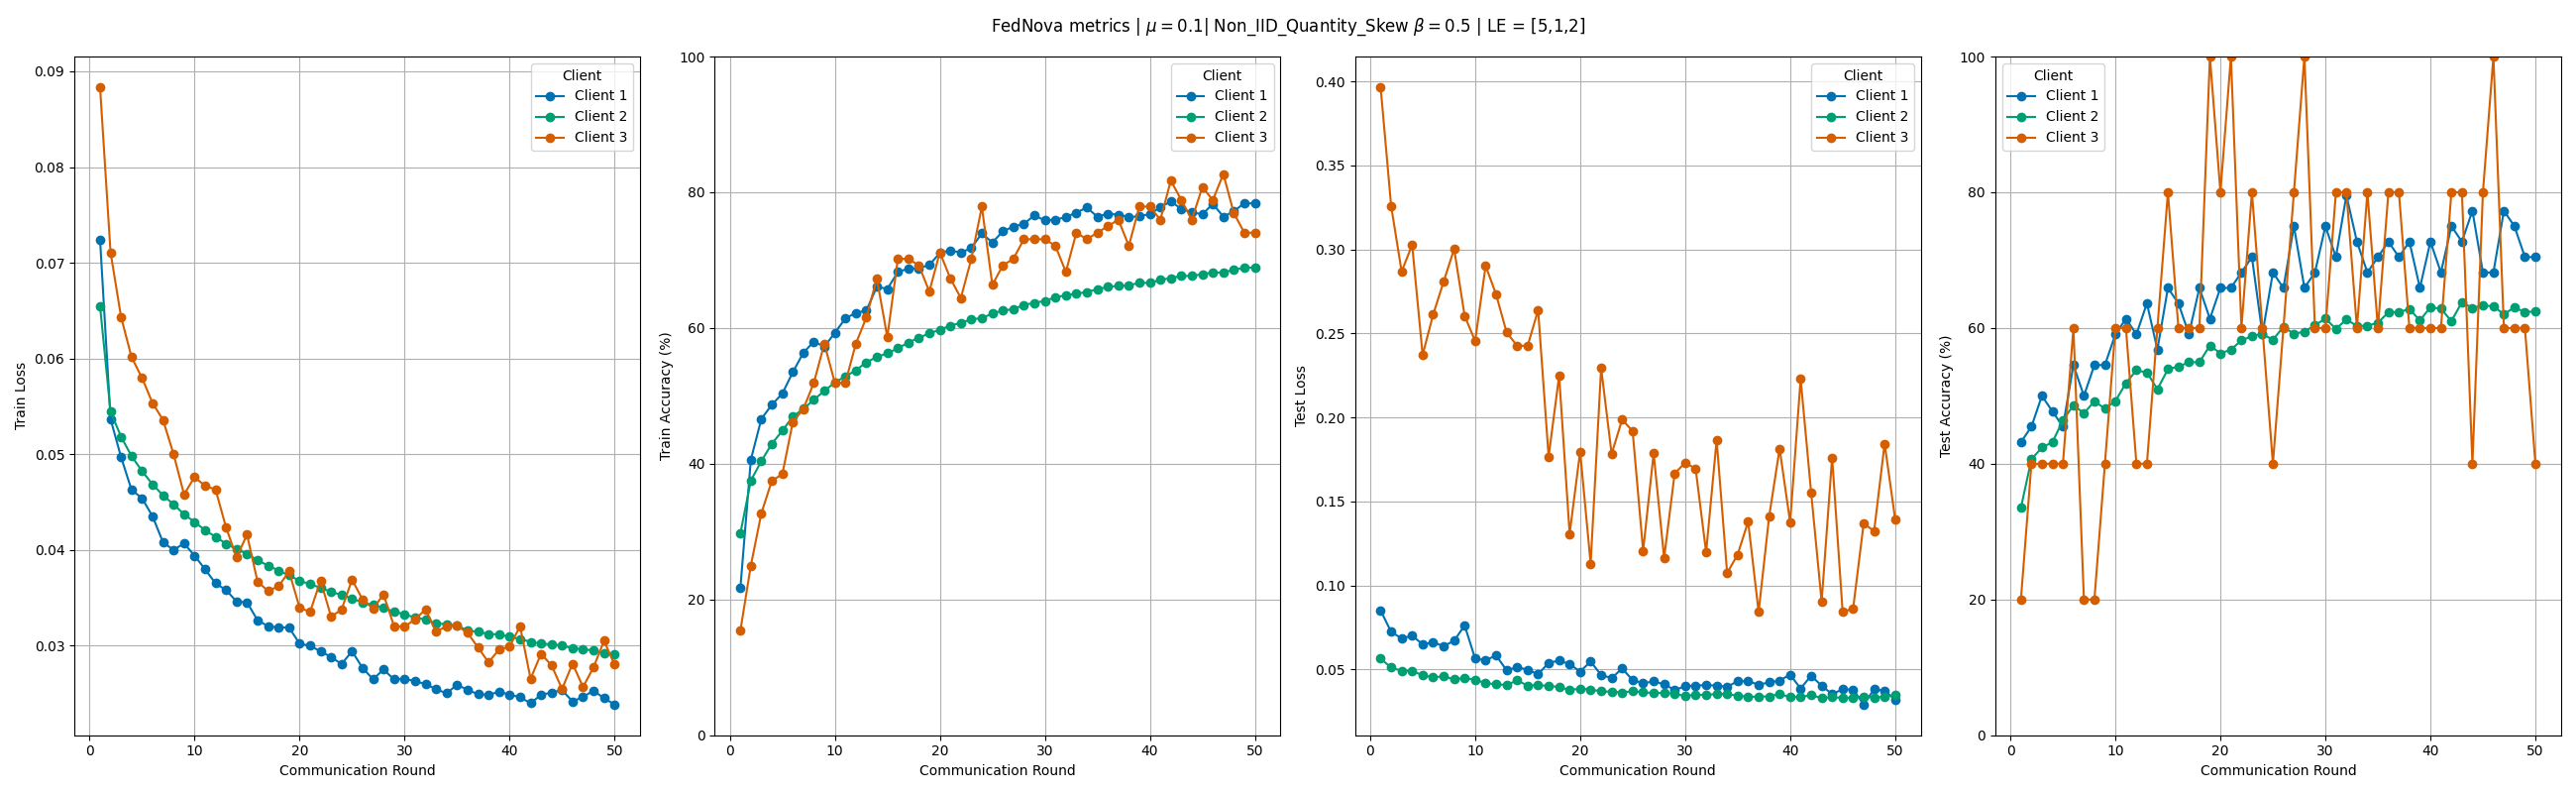
\includegraphics[width=0.9\textwidth]{figures/2-Federated_Learning/FedNova_QuantitySkew_LE_512.png}
  \caption{Local metrics for FedNova using a proximal term with $\mu=0.1$ on a Non-IID Quantity Skew setting using $Dir(\boldsymbol{\beta})$, $\boldsymbol{\beta}=(0.5,0.5,0.5)$ and local epochs [5,1,2].}
  \label{fig:FedNova_QuantitySkew_LE_512}
\end{figure}

Finally, for a feature skew experiment, we can see from Figures \ref{fig:FedNova_Noise_LE_512} and \ref{fig:FedNova_Noise_LE_512} that both approaches are similar, with FedNova having a slightly better test accuracy in all clients.
\begin{figure}[H]
  \centering
  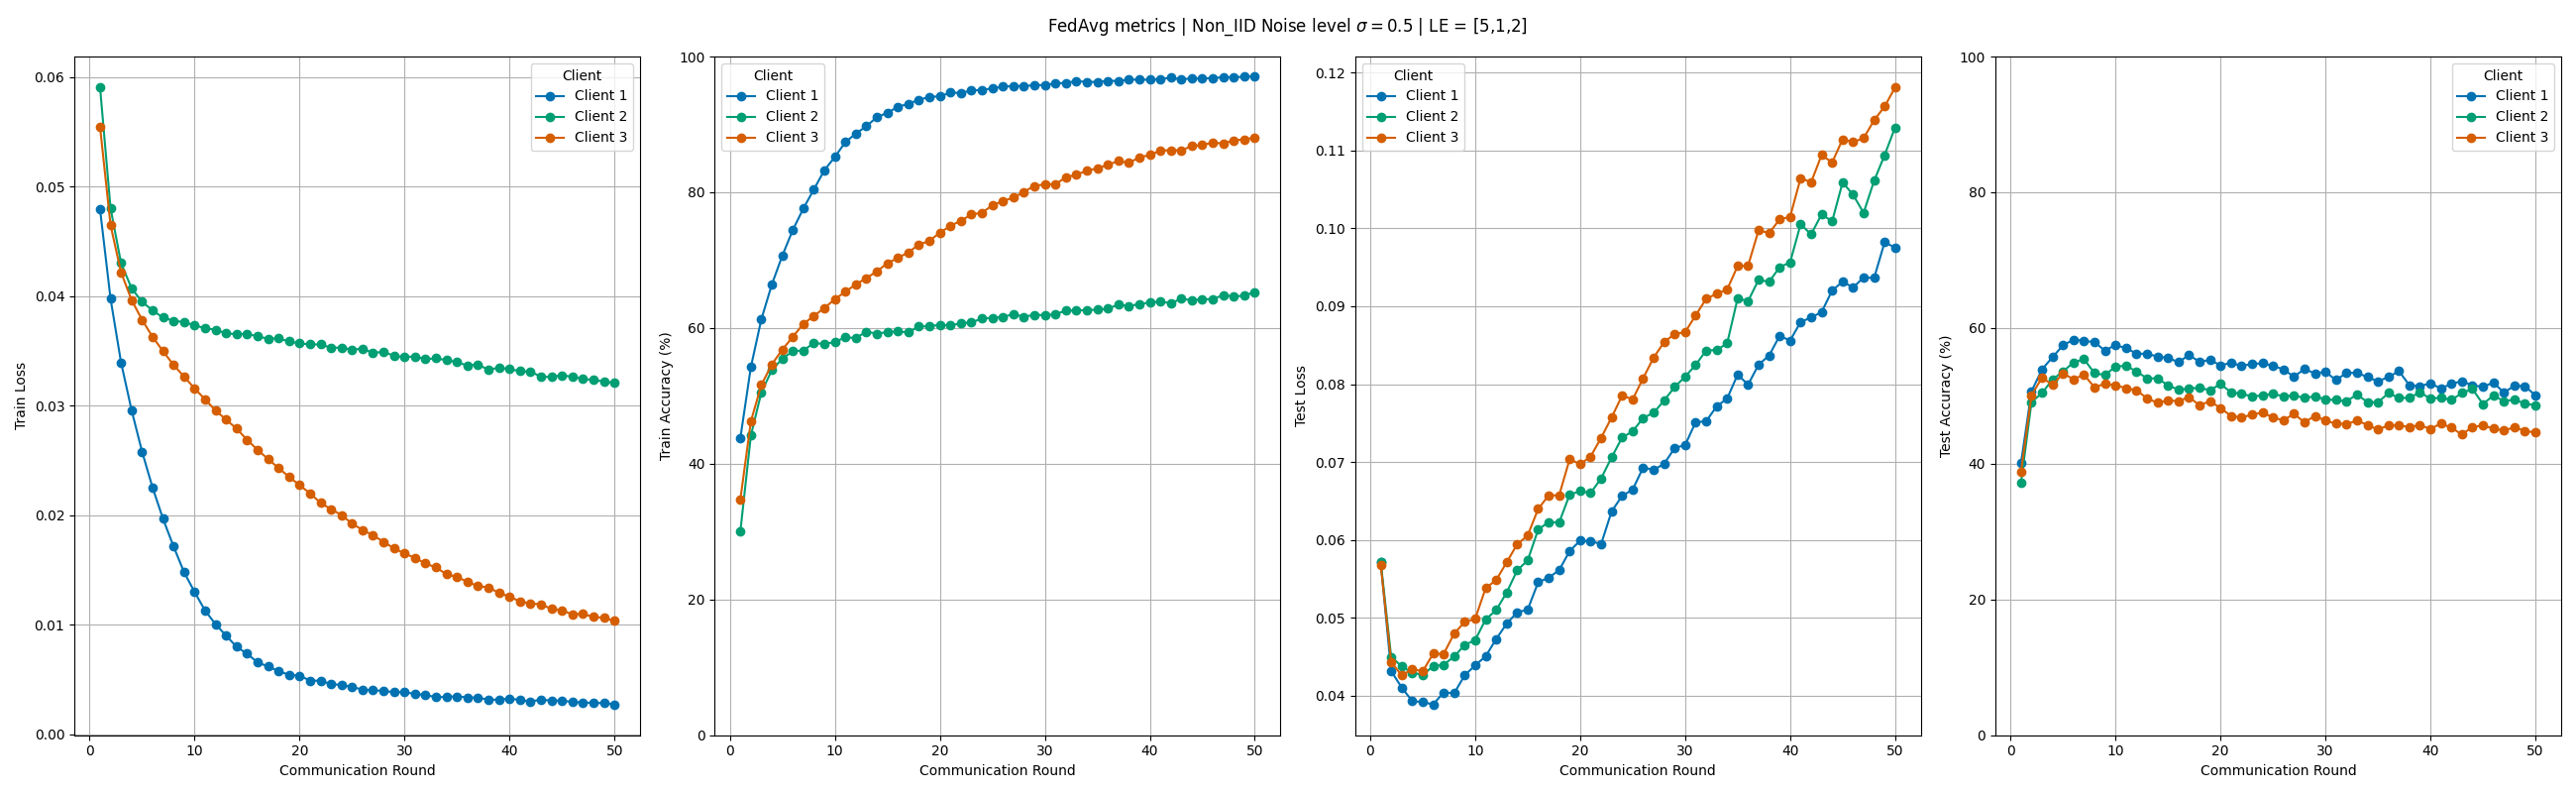
\includegraphics[width=0.9\textwidth]{figures/2-Federated_Learning/FedAvg_Noise_LE_512.png}
  \caption{Local metrics for FedAvg  on a Non-IID Feature Skew setting with noise level $\sigma=0.5$  and local epochs [5,1,2].}
  \label{fig:FedAvg_Noise_LE_512}
\end{figure}


\begin{figure}[H]
  \centering
  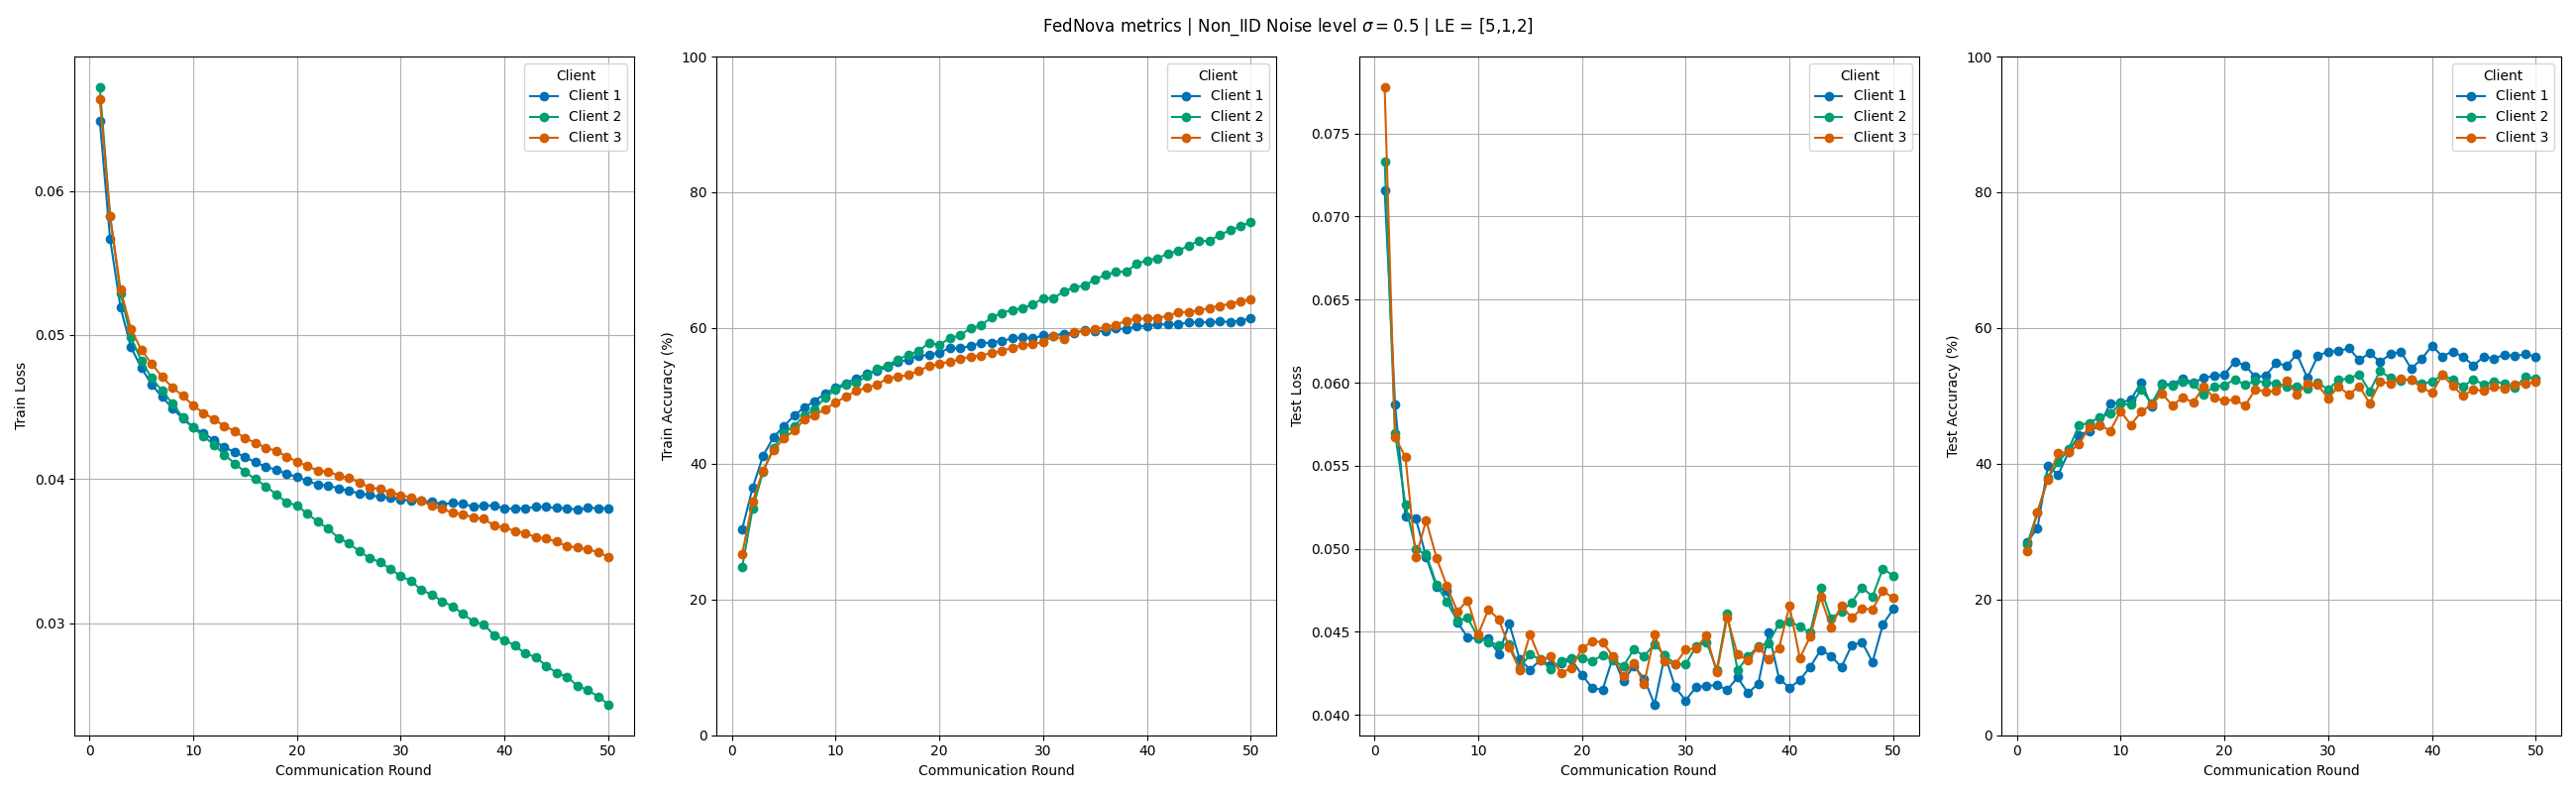
\includegraphics[width=0.9\textwidth]{figures/2-Federated_Learning/FedNova_Noise_LE_512.png}
  \caption{Local metrics for FedNova using a proximal term with $\mu=0.1$ on a Non-IID Feature Skew setting with noise level $\sigma=0.5$ and local epochs [5,1,2].}
  \label{fig:FedNova_Noise_LE_512}
\end{figure}

\begin{table}[h]
    \centering
    \begin{adjustbox}{max width=\textwidth}
    \begin{tabular}{lccccc}
        \toprule
        & IID & Label Skew Dir(0.5) & Quantity Skew Dir(0.5) & Labels per Party & Noise $\sigma=0.5$ \\
        \midrule
        FedAvg & 0.616 & \textbf{0.4328} & 0.6246 & \textbf{0.3818} & \textbf{0.5834} \\
        FedNova & \textbf{0.6231} & 0.427 & \textbf{0.6456} & 0.3552 & 0.5749 \\
        \bottomrule
    \end{tabular}
    \end{adjustbox}
    \caption{Top test accuracy obtained in FedAvg and FedNova under the same settings.}
    \label{tab:fed_comparison}
\end{table}

\begin{figure}[H]
  \centering
  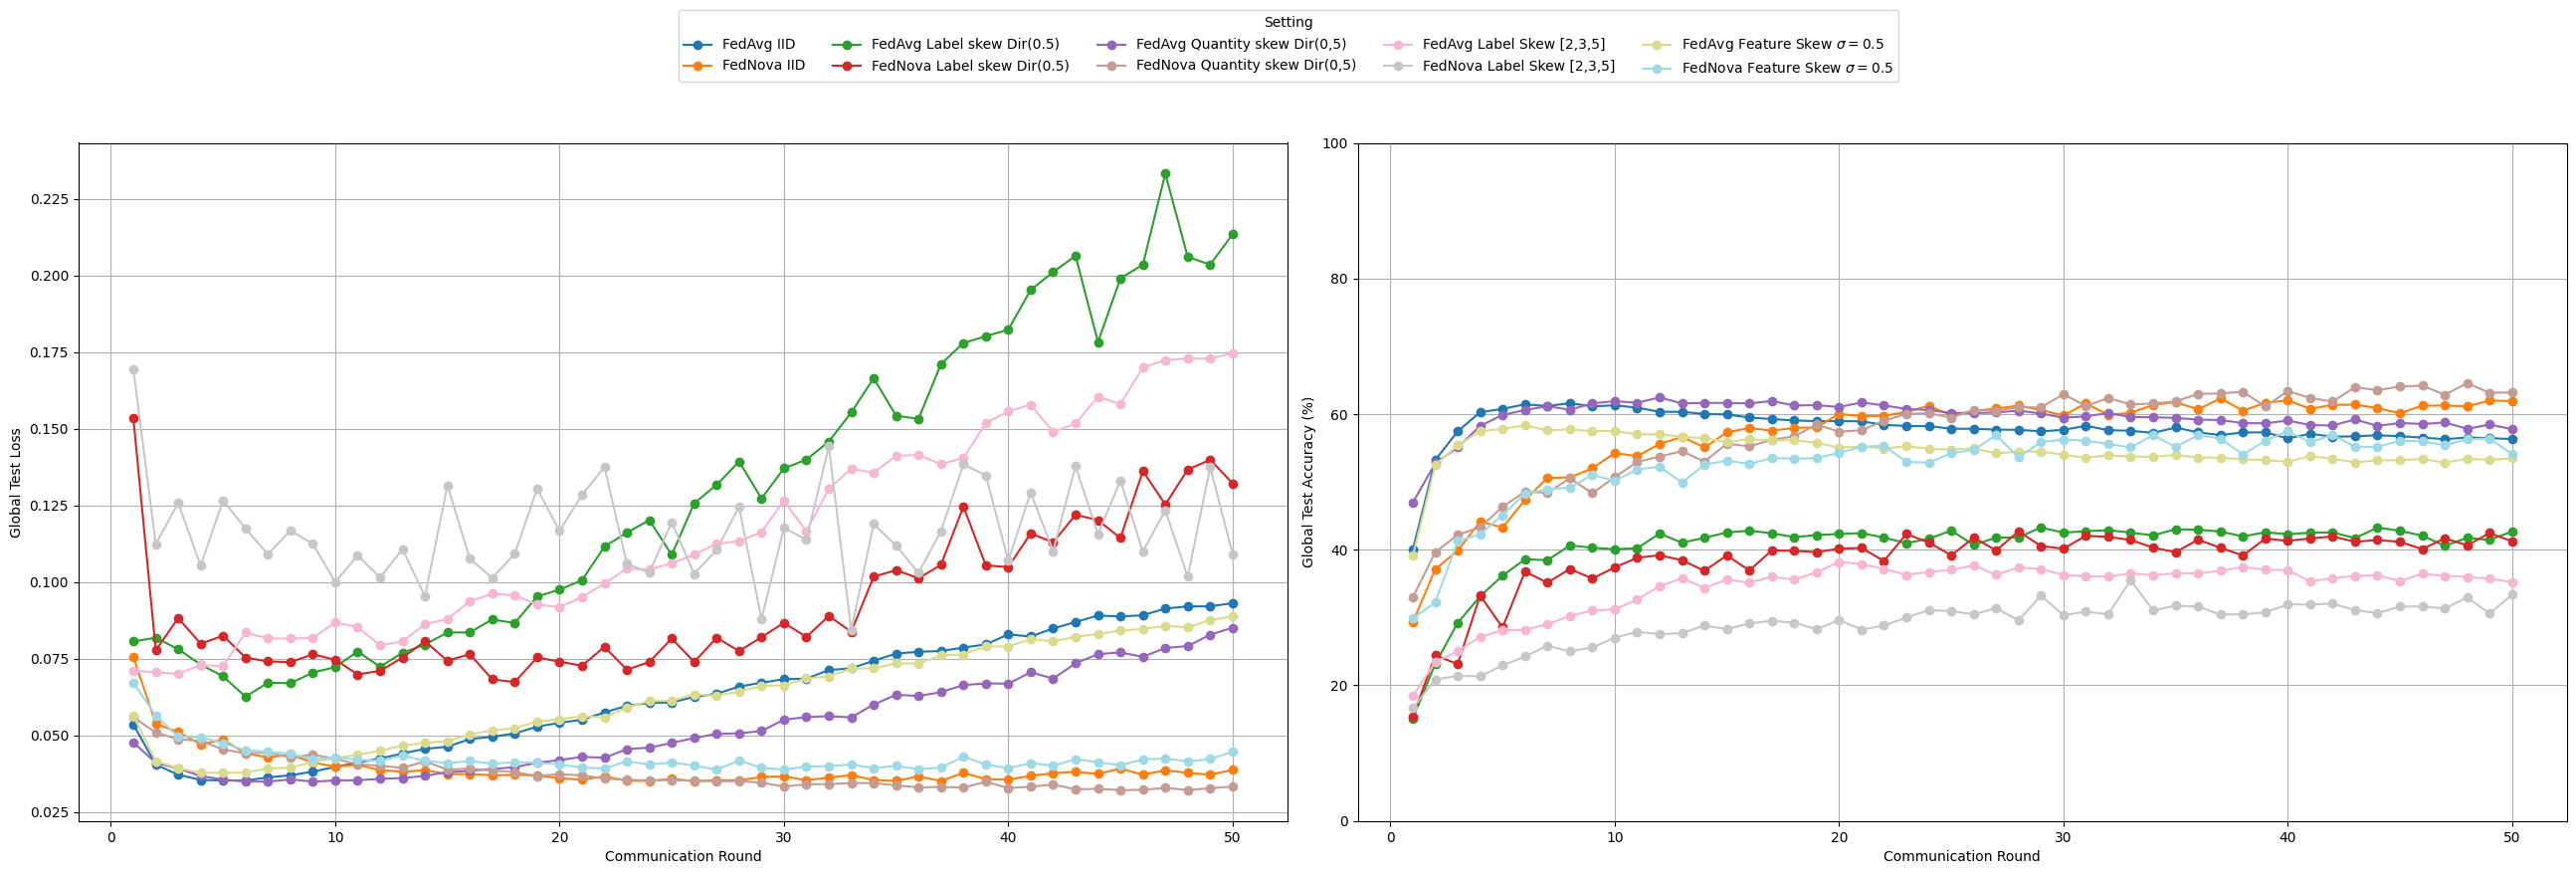
\includegraphics[width=0.9\textwidth]{figures/2-Federated_Learning/Global_Metrics_FedNova.png}
  \caption{Accuracy comparison between FedAvg and FedNova on the global test dataset.}
  \label{fig:FedNova_Global_Metrics}
\end{figure}


\section{Other algorithms to train with Non-IID data}

Among several algorithms that can be used for training a FL model under a non-IID setting, we mention some of the most performant:\\

\textbf{SCAFFOLD:}

With data heterogeneity, \textit{FedAvg} suffers from client-drift, since each local updates it's minimizing its own local objective. SCAFFOLD tries to solve this introducing control variables for the server $c$ and the clients $c_k$ $\forall k \in \{1,\dots, N\}$.

\begin{algorithm}[H]
  \label{alg:SCAFFOLD}
  \caption{SCAFFOLD}
  \begin{algorithmic}[1]
    \Require{local datasets $D^i$ $\forall i \in \{1,\dots, N\}$, number of parties $N$, number of communication rounds $T$, number of local epochs $E$, learning rate $\eta$, local mini-batch size $B$.}
    \Ensure{global model $\omega^T_g$.}
    \Statex
    \Procedure{Server execution}{}
    \State Initialize $\omega_g^0$
    \State $c^t \gets \mathbf{0}$, $c_k \gets \mathbf{0}$
    \For {round $t = 1,\dots, T$}
      \State $S_t$  (Selection of clients)
      \For {client $k \in S_t$ \textbf{in parallel}}
        \State $\Delta \omega_k^{t}, \Delta c_k \gets ClientUpdate(k, \omega_g^t, c^t)$
      \EndFor
      \State $n \gets \sum_{k \in S_t} |D^k|$
      \State $\omega_g^{t+1} \gets \omega_g^t - \eta \sum_{k \in S_t} \frac{|D^k|}{n} \Delta \omega_k^t$
      \State $c^{t+1} \gets c^t + \frac{1}{N} \sum_{k \in S_t} \Delta c_k$
    \EndFor
    \EndProcedure

    \Procedure{$ClientUpdate(k, \omega_g^t, c_k)$}{}
    \State $\omega_k^t \gets \omega_g^t$
    \State $\tau_k \gets 0$
    \State $\mathcal{B} \gets$ Batches of $D^k$ of size $B$
    \For {local epoch $i=1,\dots,E$}
      \For {batch $\mathbf{b} \in \mathcal{B}$}
        \State $\omega_k^t \gets \omega_k^t - \eta (\nabla l(\omega_k^t; \mathbf{b}) - c_k + c)$
        \State $\tau_k \gets \tau_k + 1$
      \EndFor
    \EndFor
    \State $\Delta \omega_k^t \gets \omega_g^t - \omega_k^t$
    \State $c_k^+ \gets $ (i) $\nabla l(\omega_g^t)$ or (ii) $c_k - c + \frac{1}{\tau_k \eta} (\omega_g^t - \omega_k^t)$
    \State $\Delta c \gets c_k^+ - c_k$
    \State $c_k = c_i^+$
    \State return $\Delta \omega_k^t$, $\Delta c$  to the server.
    \EndProcedure
  \end{algorithmic}
\end{algorithm}

From the SCAFFOLD's algorithm, it can be noted that the clients maintain the state of $c_k$ and the server maintain $c$, which are initialized at 0.
In comparison with the previous algorithms, here the local update formula is: $\omega_k^t = \omega_k^t - \eta (\nabla l (\omega_k^t, \mathbf{b}) - c_k + c)$. Intuitively, the local gradient $\nabla l (\omega_k^t, \mathbf{b})$ moves towards the local optimum for client $k$, the correction $c - c_k$ ensures that the update change its direction towards the global optimum.
As we can see, in line 20, there are two options for computing $c_i^+$: $\nabla l(\omega_g^t)$ or $c_k - c + \frac{1}{\tau_k \eta} (\omega_g^t - \omega_k^t)$, that is, computing the gradient of the local data at the global model or reusing the previously computed gradients. The first approach is more stable but the second one has lower computation cost.\\

\textbf{FedNAG} \cite{yang2022}: Using Nesterov Accelerated Gradient as the optimizer has proved to be a more efficient paradigm that training with FedAvg or FedSGD. For a basic description of this method see Section \ref{sec:optimizer} and Equation \ref{eqn:Nesterov_accelerated_gradient}. In the FL context, this stochastic gradient descent variant is modified as follow:\\
Let $\boldsymbol{w}_i (t)$ and $\boldsymbol{v}_i(t)$ denote the model parameter and momentum parameter in client i at $t$th iteration. Each $\tau$ iterations (local epochs) leads to a global aggregation, $t = k\tau$, $k=1,2,...$ (the original paper assumes that all clients perform the same number of local epochs). In each iteration, client $i$ performs:

\begin{align*}
  \boldsymbol{v}_i(t) &= \gamma \boldsymbol{v}_i(t-1) - \eta \nabla F_i (\boldsymbol{w}_i(t-1))\\
  \boldsymbol{w}_i(t) &= \boldsymbol{w}_i(t-1) - \gamma \boldsymbol{v}_i (t-1) + (1+\gamma) \boldsymbol{v}_i(t)\\
  &= \boldsymbol{w}_i(t-1) + \gamma \boldsymbol{v}_i(t) - \eta \nabla F_i(\boldsymbol{w}_i(t-1))
\end{align*}

In the aggregation step, the central sever performs:

\begin{align*}
  \boldsymbol{v}(t) = \frac{\sum_{i} |D^i| \boldsymbol{v}_i(t)}{\sum_j |D^j|} \\
  \boldsymbol{w}(t) = \frac{\sum_{i} |D^i| \boldsymbol{w}_i(t)}{\sum_j |D^j|}
\end{align*}

\textbf{FedADAGRAD} and \textbf{FedADAM}: Based on Adagrad optimizer explain in Equation \ref{eqn:Adagrad} and ADAM optimizer explained in equation \ref{eqn:Adam}, \cite{reddi2021} proposed an adaptive federated version of these algorithms in order to improve the convergence results of FedAvg, following its notation FedAvg's update can be expressed as:

\begin{equation*}
  \omega_g^{t+1} = \omega_g^t - \frac{1}{N} \sum_{i=1}^N (\omega_g^t - \omega_i^t)
\end{equation*}

Let $\Delta_i^t \colon = \omega_i^t - \omega_g^t$ and $\Delta_t \colon = \frac{1}{N} \sum_{i=1}^N \Delta_i^t$. The server update in FedAvg is like applying SGD to $-\Delta_t$ with learning rate $\eta=1$ (see FedOpt algorithm in \cite{reddi2021}). Therefore, the will perform the local training for each epoch $k$ computing the unbiased gradient estimate $g_{i,k}^t$ of $\nabla F_i(\omega_{i,k}^t; x)$ and updating the weights $\omega_{i,k+1}^t = \omega_{i,k}^t - \eta_l g_{i,k}^t$. After computing all local epochs of training, each client computes $\Delta_i^t = \omega_i^t - \omega_g^t$. Then, the server will get $\Delta_t = \frac{1}{N}\sum_{i=1}^N \Delta_i^t$ and the first moment estimate (with the decay parameters $\beta_1,\beta_2 \in [0,1)$) $m_t = \beta_1 m_{t-1} + (1-\beta_1)\Delta_t$. Then, adapting the optimizers from Section \ref{sec:optimizer}, FedAagrad computes the second moment estimate $v_t = v_{t-1} + \Delta_t^2$ and FedAdam $v_t = \beta_2 v_{t-1} + (1-\beta_2)\Delta_t^2$. Finally, the global model is updated $\omega_g^{t+1} = \omega_g^t + \eta \frac{m_t}{\sqrt{v_t} + \epsilon}$.
